\documentclass[a4paper, 10pt]{scrbook}  %livre

% Permet l'encodage avec le Unicode Transformation Format-8-bit
\usepackage[utf8]{inputenc}
% Permet la gestion des caractères accentués ainsi que la stabilité des impressions en P.D.F.
\usepackage[T1]{fontenc}
% Permet la stabilisation de l'écriture
\usepackage{lmodern, textcomp}
% Permet d'utiliser les liens hypertexte sans altérer la bibliothèque KOMA
\usepackage{scrhack}
\KOMAoptions{hyperref=false}
% Utilise les règles gramaticales françaises
\usepackage[french]{babel}
%Utiliser la police cal
%\usepackage[mathsrc]{eucal}
%\usepackage{eucal}
\usepackage{mathrsfs}


%Utilise les règles typographique de la bibliothéques KOMA
\setkomafont{author}{\scshape}
%\usepackage{blindtext}

% Package pour avoir plus d'arguments dans ses commandes.
\usepackage{xargs}
%Package pour plus de souplesse
\usepackage{tabularx}

%Package pour les listes indexées
\usepackage{enumitem}

%Bibliothèque mathématiques pour la police.
\usepackage{amsfonts}
%Bibliothèques mathématiques générale.
\usepackage{amsmath}
\usepackage{amssymb}
%Pour les images
\usepackage{graphicx}
%Pour appliquer \mathbb à des nombres
\usepackage{bbm}
% Pour une police grasse en math mode
\usepackage{bm}
%Package pour l'indexation de matrices
\usepackage{blkarray}
%\usepackage{dsfont}
%Package pour spreadsheet
\usepackage{spreadtab}
\usepackage{fp}
\usepackage{xstring}
\renewcommand\STprintnum[1]{\numprint{#1}}
\STsetdecimalsep{,}
\STautoround{6}
\usepackage{eurosym}
%Bibliothèque pour l'affichage de nombre avec la typographie définie
\usepackage{numprint}
\newcommand{\np}[1]{\numprint{#1}}
% Pour la notation scientifique
\usepackage{siunitx}
\sisetup{locale= FR,exponent-product=., unit-mode = text}
\DeclareSIUnit\year{ann\'{e}ee}
%Positionnement des images
\usepackage{float}
\usepackage{subcaption}
%Utilisation des couleurs
\usepackage{xcolor}
% Package pour le soulignement
\usepackage{color,soulutf8}
\setulcolor{red}
% Package pour les annotations
\usepackage{todonotes}
%\usepackage[pygments]{pythontex} % Pour utiliser Python
%\usepackage{fvextra} % Utile pour la mise en forme du code source inséré
%Package pour la programmation
\usepackage{listings}
% Package pour les scripts en R
\lstset{language=R,
    basicstyle=\small\ttfamily,
    stringstyle=\color{DarkGreen},
    otherkeywords={0,1,2,3,4,5,6,7,8,9},
    morekeywords={TRUE,FALSE},
    deletekeywords={data,frame,length,as,character},
    keywordstyle=\color{blue},
    commentstyle=\color{DarkGreen},
    }

%Définition de couleurs:
\definecolor{bleudefrance}{rgb}{.19, .55, .91}
\definecolor{pakistangreen}{rgb}{.0, .4, .0}
\definecolor{rossocorsa}{rgb}{0.83, 0.0, 0.0}
\definecolor{persimmon}{rgb}{0.93, 0.35, 0.0}
\definecolor{bronze}{rgb}{0.8, 0.5, 0.2}
% Annotation auteur
\newcommand{\Moi}[1]{\todo[color = teal!40]{#1}}
\newcommand{\Cnsl}[1]{\todo[color = pakistangreen!40]{#1}}
\newcommand{\MeG}[1]{\todo[color = rossocorsa!40]{#1}}
%Notation récurrante:
\newcommandx{\hb}[1]{\widehat{\beta_{#1}}}
\newcommandx{\prth}[4]{\left( #1_{#2} \right)_{#3\leq #2 \leq #4}}
% Encadrement des résultats
\newcommand{\enc}[1]{\fcolorbox{rossocorsa}{white}{#1}}
\newcommand{\encB}[1]{\fcolorbox{bleudefrance}{white}{#1}}
\newcommand{\encV}[1]{\fcolorbox{pakistangreen}{white}{#1}}
\newcommand{\encN}[1]{\fcolorbox{black}{white}{#1}}
% Soulignement couleur
\newcommandx{\sN}[1]{\setulcolor{black}\ul{#1}}
\newcommandx{\sR}[1]{\setulcolor{rossocorsa}\ul{#1}}
\newcommandx{\sB}[1]{\setulcolor{bleudefrance}\ul{#1}}
\newcommandx{\sV}[1]{\setulcolor{pakistangreen}\ul{#1}}
\newcommandx{\sT}[1]{\setulcolor{teal}\ul{#1}}
\newcommandx{\sO}[1]{\setulcolor{persimmon}\ul{#1}}
\newcommandx{\sG}[1]{\setulcolor{tiger}\ul{#1}}
% Text de couleur
\newcommandx{\tR}[1]{\textcolor{rossocorsa}{#1}}
\newcommandx{\tB}[1]{\textcolor{bleudefrance}{#1}}
\newcommandx{\tV}[1]{\textcolor{pakistangreen}{#1}}
\newcommandx{\tT}[1]{\textcolor{teal}{#1}}
\newcommandx{\tO}[1]{\textcolor{persimmon}{#1}}
\newcommandx{\tBr}[1]{\textcolor{bronze}{#1}}
% Écriture intervalle
\newcommandx{\inter}[2]{\left[\![#1, #2]\!\right]}
% Écriture intégrale
\newcommandx{\Su}[2]{{\displaystyle \int_{#1}^{#2}}}
% Écriture somme sigma
\newcommandx{\su}[2]{{\displaystyle \sum_{#1}^{#2}}}
% Écriture produit pi
\newcommandx{\prd}[2]{{\displaystyle \prod_{#1}^{#2}}}
%Écriture limite lim
\newcommandx{\lm}[2]{{\displaystyle \lim_{#1\to #2}}}
\DeclareMathOperator*{\argmax}{arg\,max}
\DeclareMathOperator*{\argmin}{arg\,min}
% Écriture P(X)
\newcommandx{\prob}[1]{\mathbb{P}\left(#1\right)}
% Écriture P_{\{Y\}}({X})
\newcommandx{\probC}[2]{\mathbb{P}_{#1}\left(#2\right)}
% Écriture P({X})
\newcommandx{\Prob}[1]{\mathbb{P}\left(\left\{#1 \right\}\right)}
% Écriture P_{\{Y\}}({X})
\newcommandx{\ProbC}[2]{\mathbb{P}_{\left\{#1\right\}}\left(\left\{#2\right\}\right)}
% Ecriture Esperance et Variance
\newcommandx{\E}[1]{\mathbb{E}\left(#1\right)}
\newcommandx{\Ec}[2]{\mathbb{E}_{\left\{#1\right\}}\left(#2\right)}
\newcommandx{\V}[1]{\mathbb{V}\left(#1\right)}
\newcommandx{\Vc}[2]{\mathbb{V}_{\left\{#1\right\}}\left(#2\right)}
%Symbole de la norme
\newcommandx{\norm}[1]{\left\lVert#1\right\rVert}

\title{Summarise Course/Methods}
\author{Siger}

\begin{document}

\maketitle

Si Dieu est infini, alors je suis une partie de Dieu sinon je serai sa limite\ldots

\tableofcontents
\part{Mathematical background}
\chapter{Probability's points of view}
Statistical inference lets us do 2 things:
\begin{enumerate}
	\item Estimating teh parameters of a statistical model
	\item Testing statistical hypotheses
\end{enumerate}
\section{Frequentist's point of view}
\subsection{Introduction}
This approach avoid treating parameters like random variables, and which thus avoid the 
use of priors and Bayes rule.


\subsection{Sampling distribution of an estimator}
In frequentist statistic a parameter estimate $\hat{\theta}$ is computed by applying an
estimator $\delta$ to some data $\mathcal{D}$, so $\hat{\theta}=\delta(\mathcal{D})$.
The uncertainty in the parameter estimate can be measured by computing the \emph{sampling
distribution} of the estimator.
Imagine sampling many different datasets $\mathcal{D}^{(s)}$ from some true model 
$p(\cdot|\theta^{*})$ meaning $\mathcal{D}^{(s)}=\left\{x_{i}^{(s)}\hookrightarrow 
p(\cdot|\theta^{*})\right\}_{1\leq i\leq N}$ for $1\leq s\leq S$ and $\theta^{*}$ is the 
true parameter. Now apply the estimator $\hat{\theta}(\cdot)$ to each $\mathcal{D}^{(s)}$
to get a set of estimates $\{\hat{\theta}(\mathcal{D}^{(s)})\}_{1\leq s\leq S}$.\\
As we late $S \rightarrow \infty$, the distribution induced on $\hat{\theta}(\cdot)$ is 
the \textbf{sampling distribution of the estimator}.

\paragraph{Bootstrap}
It is a simple \emph{Monte Carlo} technique to approximate the sampling 
distribution.
The idea is that if we knew the true parameters $\theta^{*}$, we could generate $S$ fake 
datasets of size $N$, from the true distribution. We could then compute our estimator from
each sample, and use the empirical distribution of the resulting samples as our estimate
of the sampling distribution.\\
Since $\theta$ is unknown, the idea of the \textbf{parametric bootstrap} is to generate
the samples using $\hat{\theta}(\mathcal{D})$ instead.
An alternative, called \textbf{non-parametric bootstrap} is to sample the $x_{i}^{s}$
(with replacement) from the original data $\mathcal{D}$ and then compute the induced
distribution as before.

\subsection{Fequentist decision theory}
In Frequentist decision theory there is a loss function and a likelihood, but there
is no prior and hence no posterior or posterior expected loss. Thus there is no 
automatic way of deriving an optimal estimator, unlike the Bayesian case.\\
Instead, we are free to choose any estimator or decision procedure $\delta: \mathcal{X}
\rightarrow \mathcal{A}$ we want.\\
Having chosen an estimator, we define its expected loss or risk as follows
\begin{center}
 $R(\theta^{*}, \delta) \triangleq \mathbb{E}_{p(\tilde{\mathcal{D}}|\theta^{*})}
\left(L(\theta^{*}, \delta(\tilde{\mathcal{D}}))\right) = \Su{}{}L\left(\theta^{*},
\delta(\tilde{\mathcal{D}})p(\tilde{\mathcal{D}})\right)d\tilde{\mathcal{D}}$   
\end{center}
where $\tilde{\mathcal{D}}$ is data sampled from 'nature's distribution' which is 
represented by parameter $\theta^{*}$.
Whereas the Bayesian posterior expected loss: 
\begin{center}
    $p(a, \mathcal{D, \pi}) \triangleq \mathbb{E}_{p(\theta|\mathcal{D},\pi)}\left(
        L(\theta, a) = \Su{\Theta}{}L(\theta, \bm{a})p(\theta|\mathcal{D}, \pi)d\theta
    \right)$
\end{center}
We see that the Bayesian approach averages over $\theta$, which is unknown, and conditions
on $\mathcal{D}$ which is known. Unlike the frequentist approach averages over $\tilde{
\mathcal{D}}$, thus ignoring the observed data, and conditions on $\theta^{*}$ which is 
unknown.

\paragraph{Bayes risk}
How to chose amongst the estimators? 
We need some way to convert $R(\theta^{*}, \delta)$ into single measure of quality, $R(
\delta)$ which does not depend on knowing $\theta^{*}$. One approach is to put a prior on
$\theta^{*}$ and then to define \textbf{Bayes risk} of an estimator as follows:
\begin{center}
    $R_{B}(\delta) \triangleq \mathbb{E}_{p(\theta^{*})}\left(R(\theta^{*}, \delta)\right)
    \Su{}{}R(\theta^{*}, \delta)p(\theta^{*})d\theta^{*}$
\end{center}
A \textbf{Bayes estimator} or \textbf{Bayes decision rule} is one which minimizes the 
expected risk: $\delta_{B} \triangleq \displaystyle\argmin_{\delta} R_{B}(\delta)$
\subparagraph{Connection Bayesian and Frequentist approaches to decision theory.}
\begin{itemize}
    \item \emph{Theorem 1} A Bayes estimator can be optained by minimizing the posterior 
        expected loss for each $\bm{x}$
    \item \emph{Theorem 2} Every admissible decision rule is a Bayes decision rule with 
        respect to some possibly improper prior distribution.
\end{itemize}
\subparagraph{Minimax risk}
Some frequentist statistic users avoid using Bayes risk since it requires the choice of
a prior, although this is only in the evaluation of the estimator, not necessarily as 
part of its construction. An alternative approach is as follows:
\begin{enumerate}
    \item Define the  maximum risk of an estimator as:\\
        $R_{max}(\delta) \triangleq \displaystyle\theta^{*}R(\bm{\theta}^{*},\delta)$
    \item A \textbf{minimax rule} is one which minimizes the maximum risk:
        $\delta_{MM} \triangleq \displaystyle\argmin_{\delta} R_{\max}(\delta)$
\end{enumerate}
Minimax estimators have a certain appeal, however computing them can be hard and 
furthermore they are very pessimistic.
In most statistical situations, excluding games theoretic ones, assuming nature is an
adversary is not a reasonable assumption.
\subparagraph{Admissible estimators}
The basic problem with frequentis decision theory is that it relies on knowing the true
distribution $p(\cdot|\theta^{*})$ in order to evaluate the risk. However it might be 
the case that some estimators are worse than others regardless of the value of 
$\theta^{*}$.\\
In particular if for $\theta \in \Theta, R(\theta, \delta_{1}) \leq R(\theta, \delta_{2})$
then we say that $\delta_{1}$ \textbf{dominates} $\delta_{2}$.\\
An estimator is said to be \textbf{admissible} if it is not strictly dominated by any 
other estimator.\\
\textbf{Admissibility is not enough}


\subsection{Desirable properties of estimators}
\subparagraph{Consistent estimators}
An estimator is said to be \textbf{consistent} if it eventually recovers the true
parameters that generated the data as the sample size goes to infinity. 

\subparagraph{Unbiased estimator}
The \textbf{bias} of an estimator is defined as 
\begin{center}
    $bias\left(\hat{\theta}(\cdot)\right) = \mathbb{E}_{p(\mathcal{D}|\theta^{*})}
    \left(\hat{\theta}(\mathcal{D})-\theta^{*}\right)$
\end{center}
The estimator is unbiased when the bias is equal to 0.

\subparagraph{Minimum variance estimators}
A famous result called the \textbf{Cramerè-Rao lower bound} provides a lower bound on the
variance of any unbiased estimator. More precisely:
Let $\left(X_{j}\right)_{1 \leq j \leq p} \hookrightarrow p(X|\theta_{0})$ and 
$\hat{\theta}(\cdot)$ an unbiased estimator of $\theta^{*}$
Then, under various smoothness assumptions on $p(X|\theta_{0})$ we have  
\begin{center}
    $\mathbb{V}(\hat{\theta}) \geq \dfrac{1}{nI(\theta^{*})}$
\end{center}
where $I(\theta^{*})$ is the Fisher information matrix.

\subparagraph{Bias-Variance Trade-off} 
As $MSE = variance + bias^{2}$\\
It might be wise to use a biased estimator, so long as it reduces our variance, assuming
our goal is to minimize squared error. 


\subsection{Empirical risk minimization}
Frequentist decision theory suffers from the fundamental problem that one cannot actually
compute the risk function, since it relies on knowing the true data distribution. By
contrast, the Bayesian posterior expected loss can always be computed since it conditions
on the data rather that on $\theta^{*}$.\\
However there is one setting which avoids this problem, it is when the task is to predict
observable quantities, as opposed to estimating hidden variables or parameters.\\
Instead of looking at loss functions of the form $L(\bm{\theta^{*}}, \delta(\mathcal{D}))$
let us look at loss functions of the form $L(y, \delta(\bm{x}))$.\\
Then the risk becomes:
$R(p_{*}, \delta) \triangleq \mathbb{E}_{(\bm{x}, y)\hookrightarrow p_{*}}\left(L(y,
\delta(\bm{x}))\right) = \su{\bm{x}}{}\su{\bm{y}}{}L(y, \delta(\bm{x}))p_{*}(\bm{x}, y)$
Where $p_{*}$ represents "nature's distribution", indeed this distribution is unknown, 
but a simple approach is to use the empirical distribution, derived from some training 
data to approximate $p_{*}$
$p_{emp} \triangleq \dfrac{1}{N}\su{i=1}{N}\delta_{x_{i}}(\bm{x})\delta_{y_{i}}(y) 
\approx p_{*}(\bm{x}, y)$
We define the empirical risk as follows:
\begin{center}
    $R_{emp}(\mathcal{D}, \mathcal{D}) \triangleq R(p_{emp}, \delta) = \dfrac{1}{N}
    \su{i=1}{N}L(y_{i}, \delta(x_{i}))$
\end{center}
\subparagraph{Regularized risk minimization}
\begin{center}
    $R'(\mathcal{D}, \delta) = R_{emp}(\mathcal{D}, \delta) + \lambda C(\delta)$
\end{center}
where $C(\delta)$ measures the complexity of the prediction function $\delta(\bm{x})$ and 
$\lambda$ controls the strength of the complexity penalty. 
This approach is known as \textbf{regularized risk minimization}.

\paragraph{Estimating the risk using cross validation}
Principle of cross validation













\subsection{Tools}
\paragraph{Introduction}
Avoid treating parameters as randome variables.
The notion of variation across repeated trials forms the basis for modelling
uncertainity.


\paragraph{Hypothesis Testing}
A \emph{frequentist} statistics, probabilities represent the frequencies at which 
particular events happen.

\paragraph{\emph{p-value}}
It is the heart of frequentist hypothesis testing, it tells us the probability of getting
a particular test statistic $t$ as big as the one we have or bigger under the null 
hypothesis (that there is actually no effect).\\
By convention we usually conclude an effect is \emph{statistically significant} if the 
\emph{p-value} is less than a threshold $\alpha$.

\paragraph{Confidence intervals}
When we fit a model to our data we look for the \emph{maximum of likelihood} parameters,
meaning the parameters that are most consistent with our data. 
For each parameter we will able to construct $95\%$ interval namely $95$ of the $100$ 
intervals generated will contain the true value of the parameter.\\
If $H_{0}: \beta=0$ is true, the probability of getting a $95\%$ confidence interval that
does not include 0 is less than 0.05. In other words, if the $95\%$ confidence does not 
include 0, $p<0.05$.
\begin{figure}[H]
	\begin{center}
		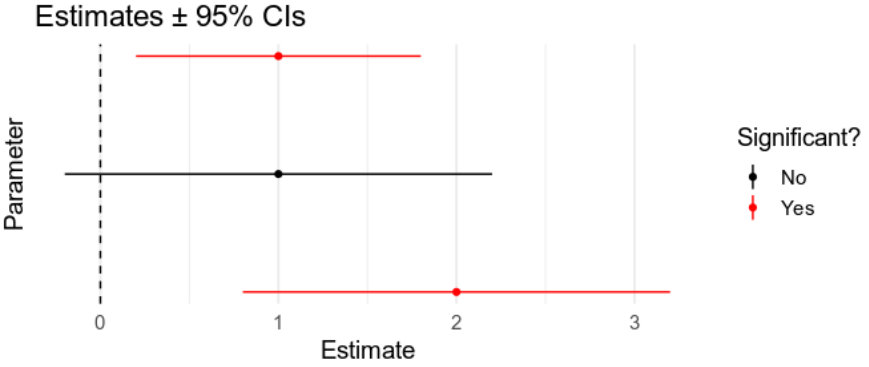
\includegraphics[width=\textwidth]{./chaps/10sec/images/4_estimates.png}
	\end{center}
	\caption{Confidence interval}
	\label{fig:4_estimates}
\end{figure}

\paragraph{Multiple comparisons}
The more tests we run the more likely it is to we'll find at least one that is significant
even though the null hypothesis is true. We can then apply a Bonferroni correction.\\
Let's say we are running $k$ tests, we can either adjust: 
\begin{itemize}
	\item the threshold $\alpha_{adj} = \dfrac{\alpha}{k}$ OR
	\item the \emph{p-value} $p_{ajd} = k\times p$
\end{itemize}


\section{Bayesian's point of view}
\subsection{Tools}

\paragraph{Summarizing posterior distributions}
\subparagraph{MAP}
Although most appropriate choice for:
$
\begin{cases}
	\text{Real valued quantity} &\rightarrow \text{\emph{posterior median or mean}}\\
	\text{Discrete} &\rightarrow \text{\emph{vector of posterior marginals}}
\end{cases}
$\\
The most popular choice is \tB{\emph{posterior mode}} aka \tR{MAP}, because it reduces to
optimization problems for which efficient algorithms often exist.\\
Some point to be aware about MAP:
\begin{itemize}
	\item \sB{No measure of uncertainty}
	\item \tB{Plugging in the MAP estimate can result in overfitting}
	\item \tB{The mode is an untypical point}, unlike the mean or median the mode is a
		point of measure 0, it does not take the volume of the space into account.
	\item \tB{MAP estimation is not invariant to reparameterization}, for example 
		passing from centimeters to inches can break things.)\\ The MLE does not
		suffer from this since the likelihood is a function not a probability
		density
\end{itemize}

\subparagraph{Credible Intervals}
With point estimates, we want a measure of confidence. 
\tB{
$$ C_{\alpha}\left(\mathcal{D}\right) = (l, u): \Prob{{l\leq \theta \leq u | \mathcal{D}}}
$$}
In general, credible intervals are usually what people want to compute but confidence
intervals are usually what they actually compute, because most people are taught 
frequentist statistics but not Bayesian statistics.\\
Sometimes with central intervals there might be points be outside the CI which have higher
probability density.\\
More formally $p^{*}$ such that: 
\begin{center}
	$1-\alpha = 
	\Su{{\theta:p(\theta|\mathcal{D})>p^{*}}}{}p(\theta|\mathcal{D})d\theta$
\end{center}
Then the \sB{HPD} such that:
\begin{center}
	$\mathcal{D}=\left\{\theta: p(\theta|\mathcal{D})\geq p^{*}\right\}$
\end{center}
\paragraph{Bayesian model selection}
A more efficient approach than cross-validation, meaning fitting \emph{k} times each
model, is to compute the posterior over models.
$$
p(m|\mathcal{D}) = \dfrac{p(\mathcal{D}|m)p(m)}{\su{{m\in\mathcal{M}}}{}p(m|\mathcal{D})}
$$
From this we can compute the \tB{MAP model $\hat{m} = \displaystyle \argmax_{m}
p(m|\mathcal{D})$}\\
Then we have the \tB{marginal likelihood}: $p(\mathcal{D}|\hat{m}) = \Su{}{}p(
\mathcal{D}|\hat{m})p(\theta|\hat{m})d\theta$
\subparagraph{Baysian Occam's razor}
In integrating out the parameters rather than maximizing them we are automatically 
protected from overfitting: model with more parameters do not necessarily have higher 
marginal likelihood.\\
A way to understand the Bayesian Occam's razor effect is to remember that probabilities 
must sum to one, meaning $\su{{\mathcal{D}'}}{}p(\mathcal{D}'|m)=1$. Complex models, which
can predict many things, must spread their probability mass thinly, and hence will not
obtain as large a probability for any given data set as simpler models.

\subparagraph{Computing the marginal likelihood (evidence)}
For a fixed model we often write:
$$p(\bm{\theta}|\mathcal{D},m) \propto p(\bm{\theta}|m)p(\mathcal{D}|\bm{\theta},m)$$
This valid since $p(\mathcal{D}|m)$ is constant. However when comparing models we need
to know how to compute the marginal likelihood, $p(\mathcal{D}|m)$. In general this can
be quite hard, since we have to integrate over all possible parameter values, but when
we have a conjugate prior, it is easy to compute.\\
Let $p(\bm{\theta})=\dfrac{q(\bm{\theta})}{Z_{0}}$ be our prior, where $q(\bm{\theta})$
is an unnormalized distribution, and $Z_{0}$ is the normalization constant of the prior.
Let $p(\mathcal{D}|\bm{\theta})=\dfrac{q(\mathcal{D}|\bm{\theta})}{Z_{l}}$ be the 
likelihood, where $Z_{l}$ contains any constant factors in the likelihood. Finally let
$p(\bm{\theta}|\mathcal{D})=\dfrac{q(\bm{\theta}|\mathcal{D})}{Z_{N}}$ be our posterior
where $q(\bm{\theta}|\mathcal{D})=q(\mathcal{D}|\bm{\theta})q(\bm{\theta})$ is the 
unnormalized posterior, and $Z_{N}$ is the normalization constant of the posterior.\\
We have:
$
\begin{cases}
	p(\bm{\theta})= \dfrac{p(\mathcal{D}|\bm{\theta})p(\bm{\theta})}{p(\mathcal{D})}\\
	\dfrac{q(\bm{\theta}|\mathcal{D})}{Z_{N}} = \dfrac{q(\mathcal{D}|\bm{\theta})
	q(\bm{\theta})}{Z_{l}Z_{0}p(\mathcal{D})}\\
	p(\mathcal{D}) = \dfrac{Z_{N}}{Z_{0}Z_{l}}
\end{cases}
$

In general $p(\mathcal{D}|m) = \Su{}{}p(\mathcal{D}|\bm{\theta})p(\bm{\theta}|m)d\bm{
\theta}$ can be quite difficult to compute. 
Simpler approach
\begin{itemize}
	\item \textbf{BIC} simple approximation:
		\tB{$BIC \triangleq \log(p(\mathcal{D}|\bm{\hat{\theta}})) - 
		\dfrac{dof(\bm{\hat{\theta})}}{2}\log(N)\approx\log{p(\mathcal{D})}$}
	\item \textbf{AIC}:
		\tB{$AIC(m,\mathcal{D})\triangleq\log(p(\mathcal{D})\bm{\hat{\theta}}_{MLE
		}) -dof(m)$}\\
		This is derived from Frequentits framework and cannot be interpreted as 
		an approximation to the marginal likelihood. The penalty of AIC is less
		than BIC, it causes AIC pick more complex models. That can be better for 
		predictive accuracy.
	\item Effect of the prior.\\
		If the prior is unknown, the correct Bayesian procedure is to put a prior
		on the prior. That is we should put a prior on the hyper-parameter 
		$\alpha$ as well as the parameters $\bm{w}$. To compute the marginal 
		likelihood we should integrate out all unknowns, we should compute:
		\tB{$\Su{}{}\Su{}{}p(\mathcal{D}|\bm{w})p(\bm{w}|\alpha,m)p(\alpha|m)
		d\bm{w}d\alpha$}
		A computational shortcut is to optimize $\alpha$ rather than integrating
		it out. That is, we use \tV{$p(\mathcal{D}|m)\approx\Su{}{}p(\mathcal{D}
		\bm{w})p(\bm{w}|\alpha,m)d\bm{w}$}.
		where \tV{$\hat{\alpha} = \displaystyle \argmax_{\alpha} p(\mathcal{D}|
			\alpha,m) = \displaystyle \argmax_{\alpha}\Su{}{}p(\mathcal{D}|
		\bm{w})p(\bm{w}|\hat{\alpha},m)d\bm{w}$}
\end{itemize}
\subparagraph{Bayes Factors}
When prior on models is uniform, then model selection is equivalent to picking the model
with the highest marginal likelihood. Now suppose we just have two models we are 
considering, call them the null hypothesis, $M_{0}$ and the alternative hypothesis,
$M_{1}$.\\
\tB{$$BF_{1,0} \triangleq \dfrac{p(\mathcal{D}|M_{1})}{p(\mathcal{D}|M_{0})}=
	\dfrac{\frac{p(M_{1}|\mathcal{D})}{p(M_{0}|\mathcal{D})}}{\frac{p(M_{1})}{
	p(M_{0})}}
$$}
This is like a likelihood ratio, except we integrate out the parameters, which allows us
to compare models of different complexity. 
\begin{table}
	\begin{tabular}{|cl|}
		\hline
	\textbf{Bayes Factor} $\bm{BF(1,0)}$ & \textbf{Interpretation}\\
		\hline
		$BF<\frac{1}{100}$ & Decisive evidence for $M_{0}$\\
		\hline
		$BF<\frac{1}{10}$ & Strong evidence for $M_{0}$\\
		\hline
		$\frac{1}{10}<BF<\frac{1}{3}$ & Modest evidence for $M_{0}$\\
		\hline
		$\frac{1}{3}<BF<1$ & Weak evidence for $M_{0}$\\
		\hline
		$1<BF<3$ & Weak evidence for $M_{1}$\\
		\hline
		$3<BF<10$ & Modest evidence for $M_{1}$\\
		\hline
		$BF>10 $ &  Strong evidence for $M_{1}$\\
		\hline
		$BF>100$ & Decisive evidence for $M_{1}$\\
		\hline
	\end{tabular}
\end{table}

\subparagraph{Jeffreys-Lindley paradox}
Problems can arise when we use improper priors (i.e. priors that do not integrate to 1)
for model selection/ hypothesis testing, even though such priors may be acceptable for 
other purposes. Thus it is important to use proper priors when doing model selection.

\paragraph{Priors}
The most controversial aspect of Bayesian statistics is its reliance on priors
\subparagraph{Uninformative priors}
If we do not have strong evidence on what $\theta$ should be, it is common to use an
uninformative priors, to "let the data speak for itself".\\
One might think that the most uninformative prior would be the uniform distribution: 
$Beta(1, 1)$, but the posterior would then be: $\E{\theta|\mathcal{D}} =
\dfrac{N_{1}+1}{N_{1}+N_{0}+2}$, whereas the MLE is $\dfrac{N_{1}}{N_{1}+N_{0}}$.\\
As by decreasing the magnitude of the pseudo counts, we can lessen the impact of the 
prior, we can argue that the most non-informative prior is: 
$$\lm{\epsilon}{0} Beta(\epsilon, \epsilon) = Beta(0, 0)$$
Called the \emph{Haldane prior}, it is an improper prior.\\
In general it is advisable to perform a some kind of sensitivity analysis, in which one
checks how much one's conclusions or prediction change in response to change in the 
modelling assumptions which includes the choice of the prior and the likelihood as well.
If the conclusion are relatively insensitive to the modelling assumption, one can have
more confidence in the results.
\subparagraph{Jeffreys priors}
Harold Jeffreys designed a general purpose technique for creating non-informative priors.
The key observation is that if $p(\phi)$ is non-informative then any re-parametrization
of the prior, such as $\theta=h(\phi)$ for some function $h$ should also be 
non-informative.
\begin{itemize}
	\item Start with a variable change: $p_{\theta}(\theta) = p_{\phi}(\phi)\left|\dfrac{d\phi}{d\theta}\right|$
	\item Consider the following constraint: $p_{\phi}(\phi)\propto
		\sqrt{\mathcal{I}(\phi)}$, where $\mathcal{I}(\phi)$ is the Fisher 
		information.\\ $\mathcal{I}(\phi) \triangleq - \E{2 \times 
		\dfrac{d\log\left(p(X|\phi)\right)}{d\phi}}$. This a measure of the
		curvature of the expected negative log likelihood and hence a measure of
		stability of the MLE.
	\item Now $\dfrac{d\log(p(x|\theta))}{d\theta} = 
		\dfrac{d\log(p(X|\phi))}{d\phi}\dfrac{d\phi}{d\theta}$
	\item $\mathcal{I}(\theta) = \mathcal{I}(\phi)
		\left(\dfrac{d\phi}{d\theta}\right)^{2}$
	\item $\sqrt{\mathcal{I}(\theta)} = \sqrt{\mathcal{I}(\phi)}\left|\dfrac{d\phi}
		{d\theta}\right|$
	\item Finally $p_{\theta}(\theta) = p_{\phi}(\phi)\left|\dfrac{d\phi}
		{d\theta}\right| \propto \sqrt{\mathcal{I}(\phi)}\left|\dfrac{d\phi}
		{d\theta}\right| = \sqrt{\mathcal{I}(\theta)}$
\end{itemize}

\subparagraph{Robust priors}
To prevent an undue influence on the result, we build priors having heavy tails, which 
avoids forcing things to be too close to the prior mean.

\subparagraph{Mixture of conjugate priors}
Conjugate priors simplify the computation of robust priors, but are often not robust, and 
not flexible enough to encode our prior knowledge. However it turns out that a mixture of
conjugate priors is also conjugate, and seem to be a good compromise.

\paragraph{Hierarchical Bayes}
A key requirement for computing the posterior $p(\theta|\mathcal{D})$ is the 
specification of a prior $p(\theta|\eta)$ where $\eta$ are the hyper-parameters. A 
Bayesian approach is to put a prior on our priors. This is an example of a \textbf{
hierarchical Bayesian Model}.

\paragraph{Empirical Bayes}
In hierarchical Bayesian models, we need to compute the posterior on multiple levels of
latent variables. For example, in a two-level model, we need to compute:
$p(\eta, \theta|\mathcal{D}) \propto p(\mathcal{D}|\theta)p(\theta|\eta)p(\eta)$\\
We can approximate the posterior on the hyper-parameters with a point-estimate, 
$p(\eta|\mathcal{D}\approx \delta_{\hat{\eta}}(\eta))$ where $\hat{\eta}=\argmax_{\eta}
p(\eta|\mathcal{D})$. Since $\eta$ is typically much smaller than $\theta$ in 
dimensionality, it is less prone to overfitting, so we can safely use a uniform prior on 
$\eta$. Then the estimate becomes: 
$$ \hat{\eta} = \argmax_{\eta} p(\mathcal{D}|\eta) = \argmax_{\eta} \Su{}{}
p(\mathcal{D}|\theta)p(\theta|\mathcal{\eta})d\theta $$
This overall approach is called \textbf{Empirical Bayes}\\
Empirical Bayes violates the principle that the prior should be chosen independently of 
the data. However, we can just view it as a computationally cheap approximation to 
inference in a hierarchical Bayesian model, just as we viewed MAP estimation as an approximation to inference in the one level model $\theta \rightarrow \mathcal{D}$. In fact, we
can construct a hierarchy in which the more integrals one performs, the "more Bayesian" 
one becomes:
\begin{center}
	\begin{tabular}{|*{2}{l|}}
		\hline
		\textbf{Method} & \textbf{Definition} \\
		\hline
		Maximum likelihood & $\hat{\theta} = \argmax_{\theta} 
		p(\mathcal{D}|\theta)$ \\
		\hline
		MAP estimation & $\hat{\theta} = \argmax_{\theta} 
		p(\mathcal{D}|\theta)p(\theta|\eta)$ \\
		ML-II (Empirical Bayes) & $\hat{\eta}=\argmax_{\eta}\Su{}{}
		p(\mathcal{D}|\theta)p(\theta|\eta)d\theta = \argmax_{\eta}p(\mathcal{D}|
		\eta)$ \\
		\hline
		MAP-II & $\hat{\eta}=\argmax_{\eta}\Su{}{}
		p(\mathcal{D}|\theta)p(\theta|\eta)p(\eta)d\theta = \argmax_{\eta}p(
		\mathcal{D}| \eta)p(\eta)$\\
		\hline
		Full Bayes & $p(\theta, \eta|\mathcal{D}) \approx p(\mathcal{D}|\theta)
		p(\theta|\eta)p(\eta)$\\
		\hline
	\end{tabular}
\end{center}

\paragraph{Bayesian decision theory}
We can formalize any given statistical decision problem as a game against nature (as 
opposed to a game against other strategic players, which is the topic of game theory).
In this game, nature picks a state or parameter or label, $y\in \mathcal{Y}$, unknown to 
us, and then generates an observation, $\bm{x}\in\mathcal{X}$ which we get to see. We then
have to make a decision, that is, we have to choose an action $a$ from some \textbf{action
space} $\mathcal{A}$.Finally we incur some \textbf{loss}, $L(y, a)$, which measures how
compatible our action $a$ is with nature's hidden state $y$.\\
Our goal is to devise a decision procedure or policy, $\delta: \mathcal{X}\rightarrow
\mathcal{A}$ which specifies the optimal action for each possible input which specifies the optimal action for each possible input, meaning the action that minimizes the expected 
loss:
$$ \delta(\bm{x}) = \argmin_{{a\in \mathcal{A}}} \E{{L(y, a)}}$$
In the Bayesian vision, the expected value of $y$ given the data we have seen so far, 
whereas in the frequentist vision the expected value refers to $x$ and $y$ that we expect
to see in the future.\\
In the Bayesian visionj the optimal action having observed $\bm{x}$ is defined as the 
action $a$ that minimizes the \textbf{posterior expected loss}:
$$ \rho(a|\bm{x})\triangleq\mathbb{E}_{p(y|x)}\left(L(y, a)\right) = \su{y}{}L(y, a)
p(y|x)$$
Hence the Bayes estimator also called Bayes decision rule is given by:
$$\delta(\bm{x}) = \argmax_{a\in\mathcal{A}}\rho(\bm{a}|\bm{x})$$

\subparagraph{Bayes estimators for common loss functions}
\begin{itemize}
	\item MAP estimate minimizes 0-1 loss: $L(y, a) = \mathbb{I}_{y\neq a}
		\begin{cases}
			0 \text{ if } a = y\\
			1 \text{ else}
		\end{cases}$
	\item Reject option, in classification problems where $p(y|\bm{x})$ is very 
		uncertain we may prefer to choose a reject action, in which we refuse to 
		classify the example as any of the specified classes. Let choosing $a=C+1$
		correspond to picking the reject action, and choosing $a\in\{1,...,C\}$
		correspond to picking one of the classes.\\
		$L(y=j, a=i) = 
		\begin{cases}
			0 &\text{ if } i=j \text{ and } i,j\in\{1,...,C\}\\
			\lambda_{r} &\text{ if } i=C+1 \\
			\lambda_{s} &\text{ otherwise}
		\end{cases} $\\
		where $\lambda_{r}$ is the cost of the reject action, and $\lambda_{s}$ is
		the cost of a substitution error. 
	\item Squared Error ($l_{2}$) for a continuous parameters. $L(y, a) = (y-a)^{2}$
	\item Absolute Error ($l_{1}$) more robust against outliers. $L(y,a)=
		\lvert y-a\rvert$. The optimal point is the median.

\end{itemize}



\paragraph{Hypothesis Testing}
A \emph{Bayesian} statistics, probabilities represent subjective beliefs. 
Bayesian hypothesis testing provides rules for calculating how you should update your 
beliefs about different hypotheses in light of the evidence you see.\\


\paragraph{Posterior belief}
We use distributions to represent model parameters, we are uncertain about.\\
We start out with \emph{prior distribution}, representing our belief before we have seen 
our data.\\
We then see some data, and the data will be more consistent with some parameters than 
others.\\
The rules of Bayesian inference tell us how to update our beliefs about the parameters now
that we've seen the data to obtain posterior beliefs.\\
Bayesian distributions are easy to interpret. The mode of the distribution is the most 
likely value of the parameter.
\begin{figure}[H]
	\begin{center}
		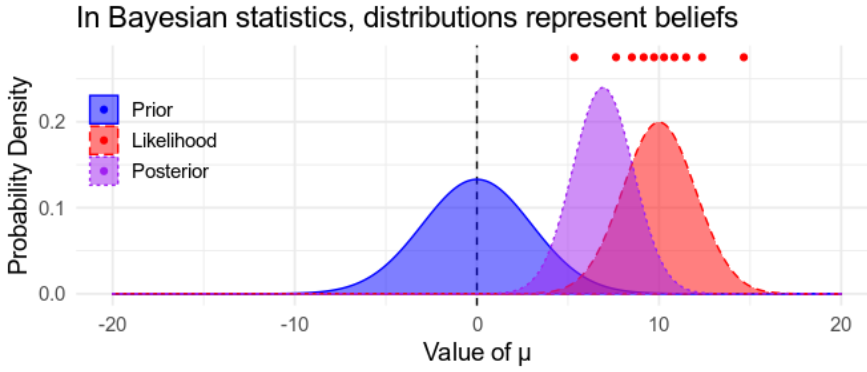
\includegraphics[width=\textwidth]{./chaps/10sec/images/2_posterior_belief.png}
	\end{center}
	\caption{Link between prior, likelihood and posterior}
	\label{fig:2_posterior_belief}
\end{figure}


\paragraph{Bayesian credible interval}
If $95\%$ of the distribution is between 2 values $\beta_{low}, \beta_{high}$ then 
according to the model there's a $95\%$ probability that the parameter is somewhere 
between these 2 values.\\
If we use uniform prior, the posterior distribution only depends on the data, and so we
end up with parameters that match the frequentist maximum-likelihood estimates: the 
posterior mode is the same as the maximum-likelihood value, and the credible intervals 
match the confidence intervals.
\begin{figure}[H]
	\begin{center}
		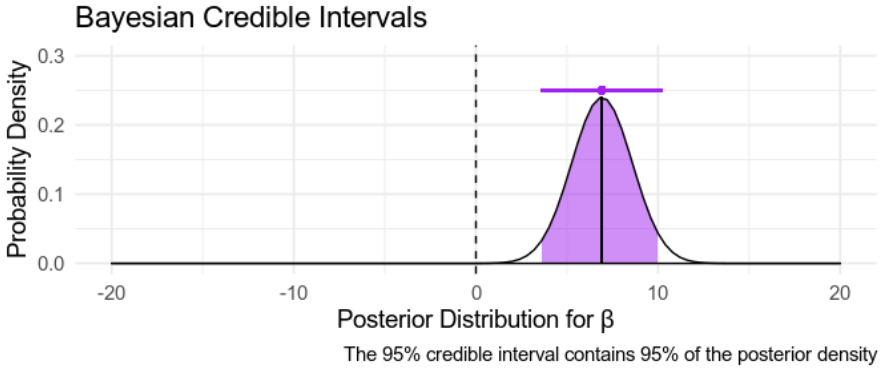
\includegraphics[width=\textwidth]{./chaps/10sec/images/1_credible_interval.png}
	\end{center}
	\caption{Bayesian Credible Intervals}
	\label{fig:1_credible_interval}
\end{figure}

\paragraph{Credible interval tests}
$95\%$ credible interval are commonly used as a simple way to decide whether an effect is
real or not: if the credible interval does not include 0, the effect is genuine. If it 
includes 0, it might not be.\\
If we use uniform prior, we can infer on the \emph{p-value}.

\paragraph{Posterior Sign tests}
Once we've calculated our posterior distribution for $\beta$, we can interrogate it 
directly. For instance if $99\%$ of the posterior distribution is above 0, we are $99\%$
sure that $\beta>0$ ($\prob{\beta>0}=0.99$) and $1\%$ sure that $\beta<0$.\\
However for example if our posterior distribution is centered on $0$ we find that 
$\prob{\beta>0}=\prob{\beta<0}=0.5$. The reason for this is that we are considering only
2 hypotheses, while ignoring that $\beta=0$. To test the hypothesis that $\beta=0$ we 
need to calculate the Bayes Factor.\\
Interestingly, the posterior sign test is closely 
\begin{figure}[H]
	\begin{center}
		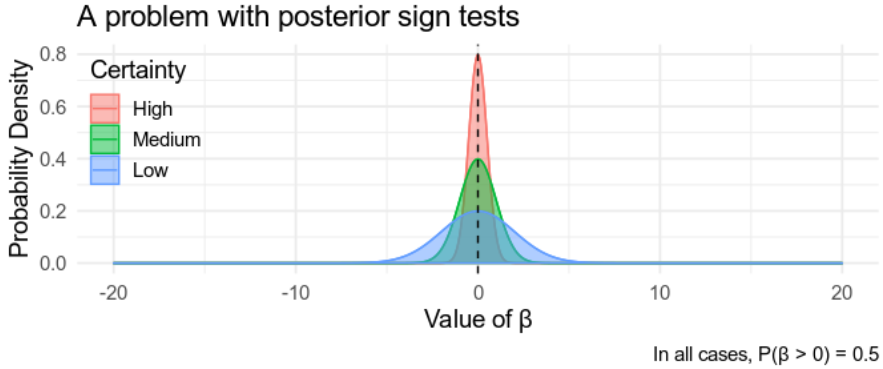
\includegraphics[width=\textwidth]{./chaps/10sec/images/3_sign_test.png}
	\end{center}
	\caption{Assessing certainty}
	\label{fig: 3_sign_test}
\end{figure}

\paragraph{Bayes Factors}
\subparagraph{Prerequisites}
$\probC{H_{0}}{Data}$ is a average over all possible values of $\beta$, weighted by how
likely each value in according to the prior.
$ \begin{cases}
	\probC{H_{1}}{Data} = \su{{i=1}}{n}\probC{\beta_{i}}{Data}\prob{\beta_{i}}\text{
		Discrete}\\
	\probC{H_{1}}{Data} = \Su{}{}\probC{\beta_{i}}{Data}\prob{\beta_{i}}\text{
		Continuous}
\end{cases} $
Setting an appropriate prior is complicated, usually initial parameters are left.

\subparagraph{Definition}
\begin{center}
	$BF_{10}=\dfrac{\probC{H_{1}}{Data}}{\probC{H_{0}}{Data}}$\\
	$BF_{01}=\dfrac{1}{BF_{10}}$\\
\end{center}
Note that in general it is easier to find evidence in favour $H_{0}$ if $H_{1}$ 
distribution is broad and easier to find evidence against $H_{0}$ if $H_{1}$ is narrow.
\begin{center}
	\begin{tabular}{|c|c|}
		\hline
		\textbf{Bayes Factor} & \textbf{Strength of evidence}\\
		\hline
		$BF=1$ & No evidence \\
		\hline
		$BF>1$ & Anecdotal evidence \\
		\hline
		$BF>3$ & Moderate \\
		\hline
		$BF>10$ & Strong \\
		\hline
		$BF>30$ & Very Strong \\
		\hline
		$BF>100$ & Extreme evidence \\
		\hline
	\end{tabular}
\end{center}

\subparagraph{Interpreting}
\textbf{Aim} : Finding how likely it is that $H_{1}$ is true and $H_{0}$ false.\\
Procedure: 
\begin{enumerate}
	\item Compute $BF_{10}$ using maximum-likelihood.
	\item Deciding how likely we thought it was the one or other hypothesis was true
		before seeing any data: \emph{the prior odds} $\prob{H_{1}}{H_{0}}$.\\
		Then there are 2 kinds of priors: prior beliefs about which hypothesis or 
		model is true, and prior beliefs about the values of the parameters in 
		each model.
	\item With the 2 above information compute the posterior distribution with Bayes'
		theorem\\ $\probC{Data}{H_{1}}=\dfrac{\probC{H_{1}}{Data}\prob{H_{1}}}{
		\probC{H_{0}}{Data}\prob{H_{0}}+\probC{H_{1}}{Data}\prob{H_{1}}}$
	\item 
\end{enumerate}
For example we get the following table:
\begin{center}
	\begin{tabular}{|*{4}{c|}}
		\hline
		$\mathbf{BF_{10}}$ & $\mathbf{BF_{01}}$ & \textbf{Prior} $\prob{H_{1}}$ &
		\textbf{Posterior} $\probC{Data}{H_{1}}$\\
		\hline
		$0.05$ & $20$ & $50\%$ & $4.8\%$\\
		\hline
		$0.1$ & $10$ & $50\%$ & $9.1\%$\\
		\hline
		$0.33$ & $3$ & $50\%$ & $25\%$\\
		\hline
		$1$ & $1$ & $50\%$ & $50\%$\\
		\hline
		$3$ & $0.33$ & $50\%$ & $75\%$\\
		\hline
		$10$ & $0.1$ & $50\%$ & $90.9\%$\\
		\hline
		$20$ & $0.05$ & $50\%$ & $95.2\%$\\
		\hline
	\end{tabular}
\end{center}


\paragraph{Multiple comparisons}
\subparagraph{Density Ratios}
\subparagraph{Posterior Estimates}
The more tests we run the more likely it is to we'll find at least one that is significant
even though the null hypothesis is true. We can then apply a Bonferroni correction.\\
Let's say we are running $k$ tests, we can either adjust: 
\begin{itemize}
	\item the threshold $\alpha_{adj} = \dfrac{\alpha}{k}$ OR
	\item the \emph{p-value} $p_{ajd} = k\times p$
\end{itemize}



\chapter{Conditional probability and Bayes' theorem}
\section{Conditional Probability}
\paragraph{Definition of a conditional probability:}
Let S be a sample space associated with a random experiment. The 
conditional probability of an event A, given that event B has occurred, is
defined by:
\begin{center}
	$\probC{B}{A}=\dfrac{\prob{A\cap B}}{\prob{B}}$
\end{center}

\section{Bayes' Theorem}
\paragraph{Law of Total Probability}
If the events $\prth{B}{i}{1}{n}$ constitute a partition of the sample
space $S$ and $\prob{B_{i}}\neq 0$ then for any event $A$ in $S$:\\
\begin{center}
	$\prob{A}=\su{i=1}{n}\prob{B_{i}}\probC{B_{i}}{A}$
\end{center}


\paragraph{Bayes'Theorem}
If the events $\prth{B}{i}{1}{n}$ constitute a partition of the sample space $S$ and
$\prob{B_{i}}\neq 0$ then for any event $A$ in $S$:\\

\begin{center}
	\enc{$\probC{A}{B_{k}} = \dfrac{\prob{B_{k}}\probC{B_{k}}{A}}{
	\su{{i=1}}{n}\prob{B_{i}}\probC{B_{i}}{A}}$}
\end{center}


\chapter{Distribution Functions}
\section{Distribution Function of Discrete Variables}
\paragraph{Definition of probability density function (pdf):}
Let $R_{X}$ be the space of the random variable $X$. The function:
$f:R_{X}\rightarrow \mathbb{R}$ defined by:
\begin{center}
	$f(x)=\Prob{X=x}$
\end{center}
is called probability density function of $X$.
\paragraph{Definition of cumulative density function (cdf):}
Let $R_{X}$ be the space of the random variable $X$. The function:
$F:R_{X}\rightarrow \mathbb{R}$ defined by:\\
\begin{center}
	$F(x)=\Prob{X\leq x}$
\end{center}
is called cumulative density function of $X$.\\Then:
\begin{center}
	$F(x)=\su{t\leq x}{{}}f(t)$
\end{center}

\section{Distribution Function of Continuous Variables}
\paragraph{Definition probability density function:}
A random variable $X$ is said to be a continuous random variable if there
exists a continuous $f:\mathbb{R}\rightarrow [0;\infty[$ such that for 
every set of real numbers $A$:
\begin{center}
	$\Prob{X\in A}=\Su{A}{{}}f(x)dx$
\end{center}
\paragraph{Definition cumulative density function:}
Let $f(x)$ be the probability density function of a continuous random
variable $X$. The cumulative distribution function $F(x)$ of $X$ is defined
as:\\
exists a continuous $f:\mathbb{R}\rightarrow [0;\infty[$ such that for 
every set of real numbers $A$:
\begin{center}
	$F(x)=\Prob{X\leq x}=\Su{-\infty}{x}f(t)dt$
\end{center}

\section{Percentile for Continuous Random Variables}
\paragraph{Definition}
Let $p\in [0;1]$, a $100p^{th}$ percentile of the distribution of a random
variable $X$ is $q\in\mathbb{R}$ satisfying:
%\begin{center}
%	$\begin{cases}\Prob{X\leq q}\leq p\\\Prob{X>q}\leq 1-p\end{cases}$
%\end{center}
\begin{center}
	$\Prob{X\leq q}\leq p$\\
	(Recall that the $F$ is a monotonically increasing function, then it has an 
	inverse $F^{-1}$)\\
	$q = F^{-1}(p)$
\end{center}
A $100p^{th}$ is a measure of location for the probability distribution in
the sense that $q$ divides the distribution of the probability mass into
2 parts, one having probability mass $p$ and other having probability mass
$1-p$
\begin{figure}[H]
	\begin{center}
		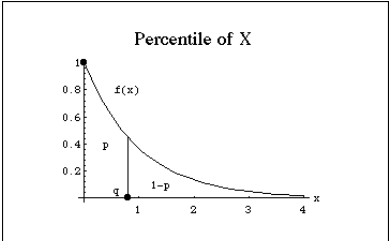
\includegraphics[width=.5\textwidth]{./chaps/12sec/images/1percentile.png}
	\end{center}
	\caption{Percentile}
	\label{fig:fig2.1}
\end{figure}
The $50^{th}$ percentile of any distribution is called median of the 
distribution.
\paragraph{Mode definition}
A mode of the distribution of a continuous random variable X is the value
of $x$ where the probability density function $f(x)$ attains a relative 
maximum.\\A mode of a random variable $X$ is one of its most probable
values.


\chapter{Moments of Random Variables and Chebychev Inequality}
\section{Moments of Random Variables}
\paragraph{$n^{th}$ moments of a random variable:}
The $n^{th}$ moment about the origin of a random variable $X$ as denoted by
$E\left( X^{n} \right)$, is defined to be:
\begin{center}
	$\E{X^{n}}=
	\begin{cases}
		\su{x\in R_{X}}{{}}x^{n}f(x)\text{ if }X\text{ is discrete}\\
		\Su{-\infty}{\infty}x^{n}f(x)dx\text{ if }X\text{ is continuous}
	\end{cases}$
\end{center}

\section{Expected Value of Random Variables}
\paragraph{Expected value:}
The expected value of a random variable $X$ as denoted by
$E\left( X \right)$, is defined to be:
\begin{center}
	$\E{X}=
	\begin{cases}
		\su{x\in R_{X}}{{}}xf(x)\text{ if }X\text{ is discrete}\\
		\Su{-\infty}{\infty}xf(x)dx\text{ if }X\text{ is continuous}
	\end{cases}$
\end{center}

\section{Variance of Random Variables}
\paragraph{Definition of Variance :}
Let $X$ be a random variable with mean $\mu_{X}$. The variance of $X$ 
denoted by $\V{X}$ or $\sigma_{X}^{2}$ is defined by:
\begin{center}
	$\V{X}=\E{\left[ X-\mu_{X} \right]^{2}}$
\end{center}
If $X$ is a random variable with mean $\mu_{X}$ and variance $\sigma_{X}^{2}$ then:
\begin{center}
$\sigma_{X}^{2}=\E{X^{2}}-\mu_{X}^{2}$
\end{center}
And:
\begin{center}
	$\V{aX+b}=a^{2}\V{X}$
\end{center}

\section{Chebychev Inequality}
\paragraph{Theorem}
Chebychev inequality allows to find an estimate of the area between the
values $\mu-k\sigma\text{ and }\mu+k\sigma$ for some given $k\neq 0$, showing
that the area under $f(x)$ on the interval $\left[\mu-k\sigma, \mu+k\sigma
\right]$ is at least $1-k^{2}$.\\
Let $X$ be a random variable with probability density function $f(x)$. If
$\mu$ and $\sigma>0$ are the mean and standard deviation of $X$ then:
\begin{center}
	\enc{$\Prob{|X-\mu|<k\sigma}\geq 1-\frac{1}{k^{2}}$}
\end{center}
\begin{figure}[H]
	\begin{center}
		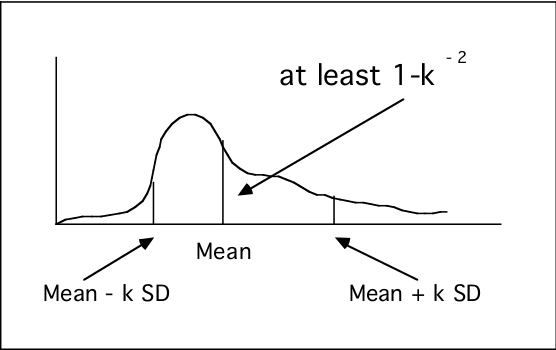
\includegraphics[width=\textwidth]{./chaps/13sec/4images/1IneqCheby.png}
	\end{center}
	\caption{Illustration of Chebychev inequality}
	\label{fig:fig2}
\end{figure}

\section{Moment Generating Funcions}
It is sometimes difficult to compute moments from the definition, a moment
generating function is a real valued function from which one can generate 
all the moment of a given random variable.
\paragraph{Definition}
Let $X$ be a random variable whose probability density function is $f(x)$.
A real valued function $M:\mathbb{R}\rightarrow\mathbb{R}$ defined by:
\begin{center}
	\enc{$M(t) = \E{e^{tX}}$}
\end{center}
if this expected value exists for all $t$ in the interval $-h<t<h$ for some
$h>0$
\paragraph{Factorial moment generating function}
FMGF of $X$ is denoted by $G(t)$ and defined as:
\begin{center}
	$G(t)=E(t^{X})$
\end{center}
$G(t)= M(\ln(t))$


%\chapter{Linear methods for Regression}
%\section{linear Regression models and Least Squares}
\subsection{Linear Regression with Mathematics point of view}
Let $X$ and $Y$ be $2$ random variables with joint pdf $f(x,y)$ and let
$h_{x}(y)$ be the conditional density of $Y$ given $\{X=x\}$\\
\begin{center}
	\enc{$\Rightarrow E_{\left\{X=x\right\}}\left(Y\right)=\Su{-\infty}{\infty}yh_{x}(y)dy$}\\ 
\end{center}
Is called the \sR{regression of $Y$ on $X$}.
\begin{itemize}
	\item
\end{itemize}

\section{Subset selection}
\begin{itemize}
	\item
\end{itemize}

\section{Shrinkage Methods}
\begin{itemize}
	\item
\end{itemize}

\section{Methods using derived input directions}
\begin{itemize}
	\item
\end{itemize}

\section{Multiple Outcome Shrinkage and Selection}
\begin{itemize}
	\item
\end{itemize}

\section{More on the Lasso and related path algorithms}
\begin{itemize}
	\item
\end{itemize}


\chapter{Important Discrete Distributions}
\section{Bernoulli Distribution}
\paragraph{Definition}
It can be thought of as a model for the set of possible outcomes of any single exp
X is the number of success during a Bernoulli process.
\begin{center}
$\forall x\in {0,1}, f(x)=p^{x}(1-p)^{1-x}\Rightarrow X\hookrightarrow$
\emph{BER}(p)
\end{center}
\paragraph{Theorem}
\begin{center}
$\begin{cases}
\mu_{X}=p\\
\sigma_{X}^{2}=p(1-p)\\
M_{X}(t)=(1-p)+pe^{t}
\end{cases}$
\end{center}

\section{Binomial Distribution}
\paragraph{Definition}
A discrete bivariate random variable $(X, Y )$ is said to have the 
bivariate binomial distribution with parameters $n, p_{1}, p_{2}$ if its
joint probability density is of the form
\begin{center}
	$f(x,y)=
	\begin{cases}	
		\dfrac{n!}{x!y!(n-x-y)}p_{1}^{x}p_{2}^{y}(1-p_{1}-p_{2})^{n-x-y}\Leftarrow (x,y)\in\mathbb{N}^{2}\\
		0\Leftarrow (x,y)\not\in\mathbb{N}^{2} 
	\end{cases}$	
	$\Rightarrow \left( X,Y \right)\hookrightarrow BIN(n,p_{1},p_{2})
	$
\end{center}
where $0<p_{1}, p_{2}, p_{1}+p_{2}<1, x+y\leq n$ and $n\geq 0$
\paragraph{Properties}
\begin{center}
	$
	\begin{cases}
	\E{X}=np_{1}\\
	\E{Y}=np_{2}\\
	\V{X}=np_{1}(1-p_{1})\\
	\V{Y}=np_{2}(1-p_{2})\\
	Cov{X,Y}=-np_{1}p_{2}\\
	M(s,t)=(1-p_{1}-p_{2}+p_{1}e^{s}+p_{2}e^{t})^{n}
	\end{cases}
	$
\end{center}
\paragraph{Conditional Properties}
\begin{center}
	$
	\begin{cases}
	\Ec{X=x}{Y}=\dfrac{p_{2}(n-x)}{1-p_{1}}\\
	\Ec{Y=y}{X}=\dfrac{p_{1}(n-y)}{1-p_{2}}\\
	\Vc{X=x}{Y}=\dfrac{p_{2}(1-p_{1}-p_{2})(n-x)}{(1-p_{1})^{2}}\\
	\Vc{Y=y}{X}=\dfrac{p_{1}(1-p_{1}-p_{2})(n-y)}{(1-p_{2})^{2}}
	\end{cases}
	$
\end{center}

\section{Geometric Distribution}
\paragraph{Definition}
\begin{center}
$\forall x\in \mathbb{N}, f(x)= (1-p)^{x-1}p\Rightarrow X\hookrightarrow\mathcal{G}(n,p)$
\end{center}
$p$ denotes the probability of success in a single Bernoulli trial
\paragraph{Theorem}
\begin{center}
$\begin{cases}
	\mu_{X}=\frac{1}{p}\\
	\sigma_{X}^{2} = \frac{1-p}{p^{2}}\\
	M_{X}(t)=\frac{pe^{t}}{1-(1-p)e^{t}}\text{ if }t<-\ln(1-p)
\end{cases}$
\end{center}
\paragraph{Memoryless property}
\begin{center}
	$X\hookrightarrow\mathcal{G}(p)\Leftrightarrow \forall(m,n)\in\mathbb{N}^{2}\ProbC{X>m}{X>m+n}
	=\Prob{X>m}$
\end{center}
The difference between the binomial and geometric distributions is in the
first the number of trials was predetermined, whereas in the last it is
the random variable.

\section{Negative Binomial Distribution}
X denotes the number of trials needed to observe the $r^{th}$ successes
$\Prob{X=x}=\Prob{\text{first }x-1\text{ trials contain: }r-1\text{ failures and }r-1\text{ successes}}\times\Prob{r^{th}\text{ success in }x^{th}\text{ trial}}$
where $p$ is the probability of success in a single Bernoulli trial.
\paragraph{Definition}
\begin{center}
	$\forall x\in \left[ r,\infty \right[, f(x)= {x-1\choose r-1}p^{r}(1-p)^{x-r}p\Rightarrow X\hookrightarrow\mathcal{NEG}(r,n)$
\end{center}
$p$ denotes the probability of success in a single Bernoulli trial
\paragraph{Theorem}
\begin{center}
$\begin{cases}
	\mu_{X}=\frac{r}{p}\\
	\sigma_{X}^{2} = \frac{r(1-p)}{p^{2}}\\
	M_{X}(t)=\left(\frac{pe^{t}}{1-(1-p)e^{t}}\right)\text{ if }t<-\ln(1-p)
\end{cases}$
\end{center}

\section{Hypergeometric Distribution}
\paragraph{Definition}
Suppose that there are $n_{1}$ objects in class $1$ and $n_{2}$ objects in
class $2$. A collection of $r$ objects is selected from these $n$ objects
at random and without replacement. We are interested in finding out the 
probability that exactly $x$ of these $r$ objects are from class $1$.
\begin{center}
	$\forall x\in \inter{0}{r}, f(x)= \frac{{n_{1}\choose x}{n_{2}\choose r-x}}{{n_{1}+n_{2}\choose r}}\Rightarrow X\hookrightarrow\mathcal{HP}(n_{1}, n_{2}, r)$
\end{center}
$p$ denotes the probability of success in a single Bernoulli trial
\paragraph{Theorem}
\begin{center}
$\begin{cases}
	\mu_{X}=r\frac{n_{1}}{n_{1}+n_{2}}\\
	\sigma_{X}^{2} = r\left(\frac{n_{1}}{n_{1}+n_{2}}\right)\left(\frac{n_{2}}{n_{1}+n_{2}}\right)\left(\frac{n_{1}+n_{2}-r}{n_{1}+n_{2}-1}\right)
\end{cases}$
\end{center}

\section{Poisson Distribution}
\paragraph{Use case}
To express the probability of a given number of events occurring in a fixed interval
of time or space if these events occur with a known constant mean rate.

\paragraph{Definition}
\begin{center}
	$\forall x\in \mathbb{N}, f(x)= \frac{e^{-\lambda}\lambda^{x}}{x!}\Rightarrow 
	X\hookrightarrow\mathcal{P}(\lambda)$
\end{center}
$\lambda\in\mathbb{R}_{+}^{*}$

\paragraph{Assumptions}
\begin{itemize}
	\item $k$ is the number of times an event occurs in an interval and 
		$k\in\mathbb{N}$
	\item Events are mutually independent.
	\item The average rate is constant.
	\item 2 events cannot occur at exactly the same instant.
\end{itemize}

\paragraph{Theorem}
\begin{center}
$\begin{cases}
	\mu_{X}=\lambda\\
	\sigma_{X}^{2} = \lambda\\
	M(t)=e^{\lambda(e^{t}-1)}
\end{cases}$
\end{center}

\section{Riemann Zeta Distribution}
\paragraph{Definition}
Initially introduced by Vilfredo Pareto to study the distribution of 
family incomes of a given country.
\begin{center}
	$\forall x\in \mathbb{N}, f(x)= \frac{1}{\zeta(\alpha+1)}x^{-\alpha+1}\Rightarrow X\hookrightarrow\mathcal{RZ}(\lambda)$
\end{center}
$\zeta(s)=\su{k=1}{\infty}\left( \frac{1}{k} \right)^{s}$ \& $\alpha > 0$
\paragraph{Theorem}
\begin{center}
$\begin{cases}
	\mu_{X}=\lambda\\
	\sigma_{X}^{2} = \lambda\\
	M(t)=e^{\lambda(e^{t}-1)}
\end{cases}$
\end{center}

\section{Pareto Distribution}
\paragraph{Definition}
Is used to model the distribution of quantities that exhibit long tails, also called heavy tails.
\begin{center}
	$\forall x\in \mathbb{N}, f(x|k,m)= km^{k}x^{-(k+1)}\mathbb{1}(x\geq m)\Rightarrow X\hookrightarrow Pareto(m, k)$
\end{center}
This density asserts that $x$ must be greater than some constant $m$, but not too much greater,
where $k$ controls what is ``too much''.
\paragraph{Theorem}
\begin{center}
$\begin{cases}
	\mu_{X}=\dfrac{km}{k-1}\\
	\sigma_{X}^{2} = \dfrac{m^{2}k}{(k-1)^{2}(k-2)}\text{ if }k>2\\
	mode = m\\
\end{cases}$
\end{center}


\chapter{Important Continuous Distributions}
\section{Uniform Distribution}
\paragraph{Definition}
A continuous bivariate random variable $(X, Y )$ is said to have
the bivariate uniform distribution with parameters on the rectangle $[a,b]\times[c,d]$ if its joint probability density is of the
form
\begin{center}
	$f(x,y)=
	\begin{cases}	
		\dfrac{1+\alpha\left( \frac{2x-2a}{b-a}-1 \right)\left( \frac{2y-2c}{d-c}-1 \right)}{(b-a)(d-c))}\Leftarrow (x,y)\in [a,b]\times[c,d]\\
		0\Leftarrow (x,y)\not\in [a,b]\times[c,d] 
	\end{cases}$	
	$\Rightarrow \left( X,Y \right)\hookrightarrow POI(p_{1},p_{2})
	$
\end{center}
where $\alpha\in [0,1]$
\paragraph{Properties}
\begin{center}
	$
	\begin{cases}
		\E{X}=\dfrac{b+a}{2}\\
		\E{Y}=\dfrac{d+c}{2}\\
		\V{X}=\dfrac{(b-a)^{2}}{12}\\
		\V{Y}=\dfrac{(d-c)^{2}}{12}\\
		Cov(X,Y)=\dfrac{1}{36}\alpha(b-a)(d-c)
	\end{cases}
	$
\end{center}
\paragraph{Conditional Properties}
\begin{center}
	$
	\begin{cases}
		\Ec{X=x}{Y}=\dfrac{d+c}{2}+\dfrac{\alpha}{6(b-a)}(c^{2}+4cd+d^{2})\left( \dfrac{2x-2a}{b-a}-1 \right)\\
		\Ec{Y=y}{X}=\dfrac{b+a}{2}+\dfrac{\alpha}{6(b-a)}(a^{2}+4ab+b^{2})\left( \dfrac{2y-2c}{d-c}-1 \right)\\
		\Vc{X=x}{Y}=\dfrac{1}{36}\left( \dfrac{d-c}{b-a} \right)^{2}\left[ \alpha^{2}(a+b)(4x-a-b)+3(b-a)^{2}-4\alpha^{2}x^{2} \right]\\
		\Vc{Y=y}{X}=\dfrac{1}{36}\left( \dfrac{b-a}{d-c} \right)^{2}\left[ \alpha^{2}(c+d)(4y-c-d)+3(d-c)^{2}-4\alpha^{2}y^{2} \right]
	\end{cases}
	$
\end{center}

\section{Gamma Distribution}
\paragraph{Gamma distribution}
The \emph{gamma} function $\Gamma(z)$ is a generalization of the notion of 
factorial, for $z\in\mathbb{R}_{+}^{*}$:\\
\begin{center}
	$\Gamma(z)=\Su{0}{\infty}x^{z-1}e^{-x}dx$
\end{center}
\subparagraph{Definition}

\begin{center}
	$f(x)\begin{cases}\frac{1}{\Gamma(\alpha)\theta^{\alpha}}x^{\alpha-1}e^{-\frac{x}{\theta}}\Rightarrow x\in\mathbb{R}_{+}^{*}\\0 \Leftarrow \overline{x\in\mathbb{R}_{+}^{*}}\end{cases}\Rightarrow X\hookrightarrow \mathcal{G}(\theta, \alpha)$
\end{center}
\subparagraph{Theorem}
$X\hookrightarrow\mathcal{\theta, \alpha}\Rightarrow
\begin{cases}
	\E{X}=\theta\alpha\\
	\V{X}=\theta^{2}\alpha\\
	M(t)=\left( \frac{1}{1-\theta t}^{\alpha}\right)\text{ if }t<\frac{1}{\theta} 
\end{cases}
$
\paragraph{Exponential distribution}
\subparagraph{Definition}
\begin{center}
	$f(x)=
	\begin{cases}
		\frac{1}{\theta}e^{-\frac{x}{\theta}}\Leftarrow x >0\\
		0\Leftarrow x\leq 0
	\end{cases}$
\end{center}
Most of the information about an exponential distribution can be obtained 
from the gamma distribution
%\subparagraph{}<++>
\paragraph{Chi-square distribution with $r$ degrees of freedom}
\subparagraph{Definition}
\begin{center}
	$f(x)=
	\begin{cases}
		\frac{1}{\Gamma{\frac{r}{2}}2^{\frac{r}{2}}}e^{-\frac{x}{2}}\Leftarrow x\in\mathbb{R}_{+}^{*}\\
		0\Leftarrow x\leq 0
	\end{cases} \Rightarrow X\hookrightarrow \chi_{2}(r)$
\end{center}
\paragraph{$n\text{-Erlang}$}
\subparagraph{Definition}
\begin{center}
	$f(x)=
	\begin{cases}
		\lambda e^{-\lambda x}\frac{(\lambda x)^{n-1}}{(n-1)!}\Leftarrow x\in\mathbb{R}_{+}^{*}\\
		0\Leftarrow x\leq 0
	\end{cases} \Rightarrow X\hookrightarrow \emph{n-Erlang}(\lambda)$
\end{center}
with $\lambda > 0$
\paragraph{Unified distribution}
\subparagraph{Definition}
\begin{center}
	$f(x)=
	\begin{cases}
		\dfrac{\alpha}{\theta^{\alpha^{\psi}}\Gamma\left( \alpha^{\psi}+1\right)}x^{\alpha -1}e^{\frac{-x^{-\left( \alpha^{\psi }- \alpha -1\right)}}{\theta}}\Leftarrow x\in\mathbb{R}_{+}^{*}\\
		0\Leftarrow x\leq 0
	\end{cases} \Rightarrow X\hookrightarrow \emph{n-Erlang}(\lambda)$
\end{center}
with $\lambda > 0$
\subparagraph{Weibull distribution}
For $\alpha = 1$ we get Weibull distribution\\
\begin{center}
$\begin{cases}\E{X}=\theta^{\frac{1}{\alpha}}\Gamma\left(1+\frac{1}{\alpha}\right)\\
	\V{X}=\theta^{\frac{2}{\alpha}}\left(\Gamma\left(1+\frac{2}{\alpha}\right)-\left(1+\frac{1}{\alpha}\right)^{2}\right)\end{cases}$
\end{center}
The Weibull distribution provides probabilistic models for life-length data of components or systems.

\section{Beta Distribution}
It is a versatile distribution and as such it is used in modeling the 
behavior of random variables that are positive but bounded in possible 
values.
\paragraph{Beta}
\subparagraph{Theorem}
Let $(\alpha,\beta)\in\mathbb{R}_{+}^{2}$ then,
\begin{center}
$B(\alpha,\beta)=\frac{\Gamma(\alpha)\Gamma(\beta)}{\Gamma(\alpha+\beta)}$\\
where $\Gamma(z)=\Su{0}{\infty}x^{z-1}e^{-x}dx$ is the gamma function
\end{center}
\subparagraph{Beta distribution}
\begin{center}
	$f(x)=\begin{cases}\frac{1}{B(\alpha,\beta)}x^{\alpha-1}(1-x)^{\beta-1}\text{, if }0<x<1\\0\text{ otherwise}\end{cases}X\hookrightarrow BETA(\alpha, \beta)$
\end{center}
\subparagraph{Beta properties}
\begin{center}
	$\begin{cases}\E{X}=\frac{\alpha}{\alpha+\beta}\\
	\V{X}=\frac{\alpha\beta}{\left(\alpha+\beta\right)^{2}(\alpha+\beta+1)}\end{cases}$
\end{center}
\paragraph{Generalized Beta}
\subparagraph{Theorem}
\begin{center}
	$f(x)=\begin{cases}f(x)=\frac{1}{B(\alpha,\beta)}\frac{(x-a)^{\alpha -1}(b-x)^{\beta -1}}{(b-a)^{\alpha + \beta - 1}}\text{ if }a<x<b\\
		0\text{ otherwise}\end{cases} \Rightarrow X\hookrightarrow GBETA(\alpha, \beta, a, b)$
\end{center}
\subparagraph{Proprieties}
\begin{center}
$\begin{cases}
	\E{X}=(b-a)\frac{\alpha}{\alpha + \beta}+a\\
	\V{X}=(b-a)^{2}\frac{\alpha\beta}{\alpha +\beta +1}
\end{cases}$
\end{center}

\section{Normal Distribution}
\paragraph{Normal Distribution}
\subparagraph{Definition}
\begin{center}
$\forall x\in\mathcal{R} f(x)=\frac{1}{\sigma\sqrt{2\pi}}e^{-\frac{1}{2}\left(\frac{x-\mu}{\sigma}\right)}\Rightarrow X\hookrightarrow\mathcal{N}(\mu,\sigma)$ 
\end{center}
\paragraph{Properties}
\begin{center}
	$\begin{cases}\E{X}=\mu\\\V{X}=\sigma^{2}\\M(t)=e^{-\mu t+\frac{1}{2}\sigma^{2}t^{2}}\end{cases}$
\end{center}
\paragraph{Chi Squared}
\subparagraph{Definition}
\begin{center}
	$X\hookrightarrow\mathcal{N}(\mu,\sigma^{2})\Rightarrow\left( \frac{X-\mu}{\sigma} \right)^{2}\hookrightarrow\chi^{2}(1)$
\end{center}

\paragraph{Generalization of normal distribution}
\begin{center}
$g(x)=\dfrac{\nu\varphi(\nu)}{2\sigma\Gamma(\frac{1}{\nu})}e^{-\left( \frac{\varphi(\nu)}{\sigma}|x-\mu| \right)^{\nu}}$ where $\varphi(\nu)=\sqrt{\dfrac{\Gamma\left(\frac{3}{\nu}\right)}{\Gamma(\frac{1}{\nu})}}$
\end{center}

\section{Lognormal Distribution}
This distribution can be defined as the distribution of a random variable
whose logarithm is normally distributed.
\paragraph{Definition}
\begin{center}
$f(x)=\begin{cases}\dfrac{1}{x\sigma\sqrt{2\pi}}e^{-\frac{1}{2}\left( \frac{ln(x)-\mu}{\sigma}\right)^{2}}\text{ if }x\in\mathbb{R}_{+}^{*}\\0\text{ otherwise}\end{cases}\Rightarrow X\hookrightarrow \wedge(\mu,\sigma)$
\end{center}
\paragraph{Properties}
\begin{center}
	$\begin{cases}\E{X}=e^{\mu+\frac{1}{2}\sigma^{2}}\\\V{X}=\left( e^{\sigma^{2}}-1 \right)e^{2\mu+\sigma^{2}}\end{cases}$
\end{center}

\section{Inverse Gaussian Distribution}
The interpurchase times of toothpaste of a family, the duration of labor 
strikes in a geographical region, word frequency in a language, conversion
time for convertible bonds, length of employee service, and crop field size
follow inverse Gaussian distribution.
\paragraph{Definition}
\begin{center}
	$f(x)=\begin{cases}\sqrt{\dfrac{\lambda}{2\pi}}x^{-\frac{3}{2}}e^{-\frac{\lambda(x-\mu)^{2}}{2\mu^{2}x}}\text{ if }x\in\mathbb{R}_{+}^{*}\\0\text{ otherwise}\end{cases}\Rightarrow X\hookrightarrow IG(\mu,\lambda)$
\end{center}
\paragraph{Properties}
\begin{center}
	$\begin{cases}
	\E{X}=\mu\\
	\V{X}=\dfrac{\mu^{3}}{\lambda}
	\end{cases}$
\end{center}

\section{Logistic Distribution}
The logistic distribution is used in modeling demographic data. It is also
used as an alternative to the Weibull distribution in life-testing.
\paragraph{Definition}
\begin{center}
	$f(x)=\dfrac{\pi}{\sigma\sqrt{3}}\dfrac{e^{-\frac{\pi}{\sqrt{3}}\left( \frac{x-\mu}{\sigma} \right)}}{\left( 1+e^{-\frac{\pi}{\sqrt{3}}\left( \frac{x-\mu}{\sigma} \right)} \right)^{2}}\Rightarrow X\hookrightarrow LOG(\mu,\sigma)$
\end{center}
\paragraph{Properties}
\begin{center}
	$\begin{cases}
		\E{X}=\mu\\
		\V{X}=\sigma^{2}\\
		M(t)=e^{\mu t}\Gamma\left( 1+\dfrac{\sqrt{3}}{\pi}\sigma t \right)\Gamma\left(1-\dfrac{\sqrt{3}}{\pi}\sigma t\right), |t|<\dfrac{\pi}{\sigma\sqrt{3}}
	\end{cases}$
\end{center}


\chapter{2 Random Variables}
\section{Bivariate Discrete Random Variables}
\paragraph{Joint probability density function}
Let $\left(X,Y\right):\left(\Omega_{X},\Omega_{Y}\right)\rightarrow\left(R_{X},R_{Y}\right)$ and $f:R_{X}\times R_{Y}\rightarrow \mathbb{R}$
\begin{center}
	$\forall (x,y)\in R_{X}\times R_{Y},f(x,y)=\Prob{X=x,Y=y}\Leftrightarrow\text{ f is the joint probability density function for }X\text{ and }Y$
\end{center}
\paragraph{Marginal probability density function}
Let for all $(x,y)\in R_{X}\times R_{Y}$: $f(x,y)$ be the joint probability density of $X$ and $Y$
\begin{center}
$\begin{cases}
	f_{1}(x)=\su{ {y\in R_{y}}}{}f(x,y)\text{is the marginal probability density of }X\\
	f_{2}(y)=\su{ {x\in R_{x}}}{}f(x,y)\text{is the marginal probability density of }Y
\end{cases}$
\end{center}
\paragraph{Joint cumulative probability distribution function}
Let $F:\mathbb{R}^{2}\rightarrow\mathbb{R}$
\begin{center}
	$\forall (x,y)\in \mathbb{R}^{2},F(x,y)=\Prob{X\leq x,Y\leq y}\Leftrightarrow\text{ F is the joint cumulative probability density function for }X\text{ and }Y$
\end{center}

\section{Bivariate Continuous Random Variables}
\paragraph{Marginal probability density function}
Let for all $(x,y)\in R_{X}\times R_{Y}$: $f(x,y)$ be the joint probability density of $X$ and $Y$
\begin{center}
$\begin{cases}
	f_{1}(x)=\Su{{-\infty}}{\infty}f(x,y)dy\text{is the marginal probability density of }X\\
	f_{2}(y)=\Su{{-\infty}}{\infty}f(x,y)dx\text{is the marginal probability density of }Y
\end{cases}$
\end{center}
\paragraph{Joint cumulative probability distribution function}
Let $F:\mathbb{R}^{2}\rightarrow\mathbb{R}$
\begin{center}
	$\forall (x,y)\in \mathbb{R}^{2},F(x,y)=\Prob{X\leq x,Y\leq y}=\Su{ {-\infty}}{y}\Su{ {-\infty}}{x}f(u,v)dudv\Leftrightarrow\text{ F is the joint cumulative probability density function for }X\text{ and }Y$
\end{center}
From the fundamental theorem of calculus:
$f(x,y)=\dfrac{\partial^{2}F(x,y)}{\partial x\partial y}$

\section{Conditional Distributions}
Keeping previous notations:
\paragraph{Conditional probability density function}
The conditional probability density function $g$ of $X$ given the event
$\left\{ Y=y \right\}$ is defined as 
\begin{center}
	$g_{ \{Y=y\}}(x)=\dfrac{f(x,y)}{f_{2}(y)}$
\end{center}

\section{Independence of Random Variables}
The random variables $X$ and $Y$ are (stochastically) independent if and only if
\begin{center}
	$\forall (x,y)\in R_{X}\times R_{Y}, f(x,y)=f_{1}(x)f_{2}(y)$
\end{center}

\paragraph{Conditionally independent}
Usually, in a set of variables, the unconditional independence is rare, because most 
variables can influence most variables, however the influence is mediated via other 
variables rather than being direct. We therefore say $X$ and $Y$ are conditionnally
independent given $Z$ if
\begin{center}
	$\probC{Z}{X} = \probC{Z}{X}\probC{Z}{Y}$\\
	or\\
	$f_{x,y}(x,y|z) = f_{x}(x|z)\times f_{y}(y|z)$
\end{center}


\chapter{Product Moments of Bivariate Random Variabless}
\section{Covariance of Bivariate Random Variables}
\paragraph{Product Moment}
The product moment of $X$ and $Y$, denoted $\E{XY}$ is defined as:
\begin{center}
	$\begin{cases}
		\su{ {x\in R_{X}}}{}\su{ {y\in R_{Y}}}{}xyf(x,y)\text{ if }X\text{ and } Y\text{ are discrete}\\
		\Su{ {-\infty}}{\infty}\Su{ {-\infty}}{\infty}xyf(x,y)dxdy\text{ if }X\text{ and } Y\text{ are continuous}
	\end{cases}$
\end{center}
\paragraph{Covariance}
\subparagraph{Definition}
Let $X$ and $Y$ 2 random variables with joint density function $f$:
\begin{center}
	$Cov\left( X,Y \right)=\E{\left( X-\mu_{X} \right)\left( Y-\mu_{Y} \right)}= \E{XY}-\E{X}\E{Y}$
\end{center}
\subparagraph{Properties}
\begin{center}
	$Cov(aX+b, cY+d)=acCov(X,Y)$
\end{center}

\section{Independence of Random Variables}
\paragraph{Properties}
\begin{center}
	$\begin{cases}
	X\&Y: independent \Rightarrow \E{XY}=\E{X}\E{Y}\\
	X\&Y: independent \Rightarrow Cov(X,Y)=0
	\end{cases}$
\end{center}

\section{Variance of Linear Combination Random Variables}
\subparagraph{Properties}
\begin{center}
	$\begin{cases}
	X,Y: 2 RV \Rightarrow \V{aX+bY}=a^{2}\V{X}+b^{2}\V{Y}+2abCov(X,Y)\\
	X,Y: independent \Rightarrow \V{XY}=\V{X}\V{Y}	
	\end{cases}$
\end{center}

\section{Correlation and Independence}
\paragraph{Correlation coefficient}
To get correlation coefficient: convert each variable to standard units
and compute the average of their product.
\begin{center}
	$X,Y\text{: 2 RV}\Rightarrow \rho=\dfrac{Cov(X,Y)}{\sigma_{X}\sigma_{Y}}$
\end{center}
\begin{figure}[H]
	\begin{center}
		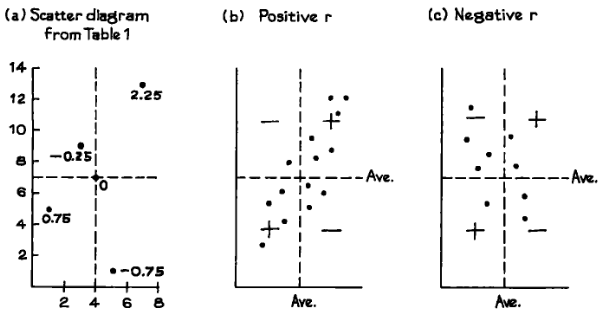
\includegraphics[width=.5\textwidth]{./chaps/17sec/images/correlationDiagram.png}
	\end{center}
	\caption{+: area where r is positive.\\-: area where r is 
	negative}
	\label{fig:7_correlationDiagram}
\end{figure}
Associated with each of one SD in $x$ there is an increase of only
$r$ SDs in $y$, on the average.
\begin{figure}[H]
	\begin{center}
		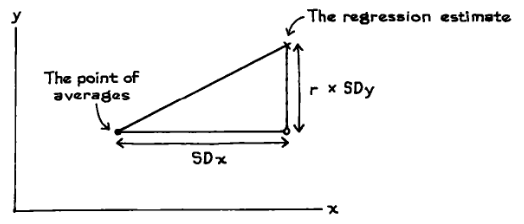
\includegraphics[width=.5\textwidth]{./chaps/17sec/images/2_correlDiag.png}
	\end{center}
	\caption{Graphical representation of $r$}
	\label{fig:2_correDiag}
\end{figure}
\begin{figure}[H]
	\begin{center}
		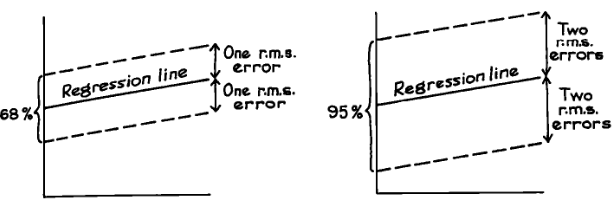
\includegraphics[width=.5\textwidth]{./chaps/17sec/images/3_residuals.png}
	\end{center}
	\caption{Graphical interpretation of Residual Mean Squares}
	\label{fig:3_rmsDiag}
\end{figure}
\paragraph{Property}
\begin{center}
	$X,Y\text{: 2 RV}\Rightarrow -1\leq \rho \leq 1$
\end{center}


\section{Moment Generating Function}
One can define the moment generating function for the bivariate case to
compute the various product moments
\paragraph{Moment generating function}
Let $X$ and $Y$ be 2 random variables with joint density
function $f(x,y)$. A real valued function $M: \mathbb{R}^{2}\rightarrow\mathbb{R}$
\begin{center}
	$\forall (t,s)\in[-k,k]\times[-h,h]M(s,t)=\E{e^{sX+tY}} exists\Rightarrow M\text{ is the joint moment generating function of }X\text{ and }Y$
\end{center}
\paragraph{Property}
\begin{center}
	$X,Y\text{: independent}\Rightarrow M_{aX+bY}(t)=M_{X}(at)M_{Y}(bt)$
\end{center}



\chapter{Conditional Expectation of Bivariate Random Variables}
\section{Conditional Expected Values}
\paragraph{Conditional expectation}
The conditional mean of $X$ given $Y=y$ is defined as:
\begin{center}
\enc{
$
\E{X|y}=
\begin{cases}
\su{{x\in R_{X}}}{}xg(x/y)\Leftarrow X\text{ discrete}\\
\Su{{-\infty}}{\infty}xg(x/y)dx\Leftarrow X\text{ continuous}
\end{cases}
$}
\end{center}

\paragraph{Properties}
\begin{center}
	$\begin{cases}
		\mathbb{E}_{X}\left( \Ec{{y|x}}{{Y|X}} \right)=\Ec{y}{Y}\\
	\E{Y|\left\{ X=x \right\}}=\mu_{Y}+\rho\dfrac{\sigma_{Y}}{\sigma_{X}}(x-\mu_{X})
	\end{cases}$	
\end{center}

\section{Conditional Variance}
\paragraph{Definition}
\begin{center}
	$\begin{cases}
	\V{Y|x}=\E{Y^{2}|x}-\E{Y|x}^{2}\\
	\mathbb{E}_{x}\left( \V{Y|X}=(1-\rho^{2})\V{Y} \right)
	\end{cases}$
\end{center}

\section{Regression Curve and Scedastic Curves}
\paragraph{Regression function of $Y$ on $X$}
\begin{center}
	$\E{Y|\left\{ X=x \right\}}=\Su{ {-\infty}}{\infty}yh(y/x)dx$
\end{center}
The graph of this regression function of $Y$ on $X$ is known as the 
regression curve of $Y$ on $X$.
\paragraph{Linear regression}
Let X and Y be two random variables with joint probability density function
$f(x, y)$ and let $\E{Y |\left\{ X = x \right\}}$ be the regression function of Y
on X. If this regression function is linear, then $\E{Y |\left\{ X = x \right\}}$ is called a linear
regression of Y on X. Otherwise, it is called nonlinear regression of Y on X.
\paragraph{Scedastic function}
Let $h(y/x)$ is the conditional density of Y given $\left\{ X=x \right\}$
\begin{center}
	$\V{Y|\left\{ X=x \right\}}=\Su{ {-\infty}}{\infty}y^{2}h(y/x)dy$
\end{center}
The graph of this scedastic function of Y on X is known as the scedastic
curve of Y on X


\chapter{Functions of Random Variables and Their Distribution}
%\section{Distribution Function Method}
%\begin{itemize}
	\item
\end{itemize}

\section{Transformation Method for Univariate Case}
The most useful method to find the probability density function of a 
transformed random random variable.
\begin{center}
S'exercer sur pdf p276
\end{center}
\paragraph{Essential theorem for transforming}
Let X be a continuous random variable with probability density function 
$f(x)$. Let $y=T(x)$ be an increasing (or decreasing) function.
Then the density function of the random variable $Y = T(X)$ is given by
\begin{center}
$g(y)=\left|\dfrac{dx}{dy}\right|f\left( W(y) \right)$
\end{center}
where $W$ is the inverse function of $T$

\section{Transformation Method Bivariate Case}
\paragraph{Essential theorem to method of bivariate case}
Let $X$ and $Y$ be $2$ continuous random variables with joint density $f(x, y)$. Let $U=P(X,Y)$ and $V = Q(X,Y)$ be functions of $X$
and $Y$ . If the functions $P(x,y)$ and $Q(x,y)$ have single valued inverses, say
$X=R(U,V)$ and $Y=S(U,V)$, then the joint density $g(u,v)$ of $U$ and $V$ is given by
\begin{center}
	$g(u,v)=|J|f\left(R(u,v),S(u,v)\right)$
\end{center}
where $J=
\begin{vmatrix}
	\dfrac{\partial x}{\partial u} & \dfrac{\partial x}{\partial v}\\
	\dfrac{\partial y}{\partial u} & \dfrac{\partial y}{\partial v}
\end{vmatrix}
=\dfrac{\partial x}{\partial u}\dfrac{\partial y}{\partial v}-\dfrac{\partial x}{\partial v}\dfrac{\partial y}{\partial u}$
\paragraph{Density functions}
Let the joint density of the random variables $X$ and $Y$ be $Y$
$f(x, y)$. Then probability density functions of $X + Y$ , $XY$ , and $\dfrac{X}{Y}$ are given by
\begin{center}
$\begin{cases} 
	h_{X+Y}(v) = \Su{ {-\infty}}{\infty}f(u,v-u)du\\
	h_{XY}(v) = \Su{ {-\infty}}{\infty}\dfrac{1}{|u|}f(u,\frac{v}{u})du\\
	h_{X+Y}(v) = \Su{ {-\infty}}{\infty}|u|f(u,vu)du
\end{cases}$
\end{center}

\section{Convolution Method for Sums of Random Variables}
\paragraph{Definition of convolution}
Let $f$ and $g$ be $2$ real valued function. The convolution of $f$ and $g$is defined as:
\begin{align*}
	(f*g)(z)=&\Su{ {-\infty}}{\infty}f(z-y)g(y)dy\\
	=& \Su{ {-\infty}}{\infty}g(z-x)f(x)dx
\end{align*}
Thus thanks to the previous theorem, if $X\text{ and }Y$ are 2 independent RV then $f*g$ is the density of the random variable $Z= X+Y$ 

\section{Moment Method for Sums of Random Variables}
This method is based on the fact that:
\begin{center}
	$M_{X+Y}(t)=M_{X}(t)\times M_{Y}(t)$
\end{center}


\chapter{Some Special Discrete Bivariate Distributions}
\section{Bivariate Bernoulli Distribution}
\paragraph{Definition}
It can be thought of as a model for the set of possible outcomes of any single exp
X is the number of success during a Bernoulli process.
\begin{center}
$\forall x\in {0,1}, f(x)=p^{x}(1-p)^{1-x}\Rightarrow X\hookrightarrow$
\emph{BER}(p)
\end{center}
\paragraph{Theorem}
\begin{center}
$\begin{cases}
\mu_{X}=p\\
\sigma_{X}^{2}=p(1-p)\\
M_{X}(t)=(1-p)+pe^{t}
\end{cases}$
\end{center}

\section{Bivariate Binomial Distribution}
\paragraph{Definition}
A discrete bivariate random variable $(X, Y )$ is said to have the 
bivariate binomial distribution with parameters $n, p_{1}, p_{2}$ if its
joint probability density is of the form
\begin{center}
	$f(x,y)=
	\begin{cases}	
		\dfrac{n!}{x!y!(n-x-y)}p_{1}^{x}p_{2}^{y}(1-p_{1}-p_{2})^{n-x-y}\Leftarrow (x,y)\in\mathbb{N}^{2}\\
		0\Leftarrow (x,y)\not\in\mathbb{N}^{2} 
	\end{cases}$	
	$\Rightarrow \left( X,Y \right)\hookrightarrow BIN(n,p_{1},p_{2})
	$
\end{center}
where $0<p_{1}, p_{2}, p_{1}+p_{2}<1, x+y\leq n$ and $n\geq 0$
\paragraph{Properties}
\begin{center}
	$
	\begin{cases}
	\E{X}=np_{1}\\
	\E{Y}=np_{2}\\
	\V{X}=np_{1}(1-p_{1})\\
	\V{Y}=np_{2}(1-p_{2})\\
	Cov{X,Y}=-np_{1}p_{2}\\
	M(s,t)=(1-p_{1}-p_{2}+p_{1}e^{s}+p_{2}e^{t})^{n}
	\end{cases}
	$
\end{center}
\paragraph{Conditional Properties}
\begin{center}
	$
	\begin{cases}
	\Ec{X=x}{Y}=\dfrac{p_{2}(n-x)}{1-p_{1}}\\
	\Ec{Y=y}{X}=\dfrac{p_{1}(n-y)}{1-p_{2}}\\
	\Vc{X=x}{Y}=\dfrac{p_{2}(1-p_{1}-p_{2})(n-x)}{(1-p_{1})^{2}}\\
	\Vc{Y=y}{X}=\dfrac{p_{1}(1-p_{1}-p_{2})(n-y)}{(1-p_{2})^{2}}
	\end{cases}
	$
\end{center}

\section{Bivariate Geometric Distribution}
\paragraph{Definition}
A discrete bivariate random variable $(X, Y )$ is said to have
the bivariate Geometric distribution if its joint probability density is of the
form
\begin{center}
	$f(x,y)=
	\begin{cases}	
		\dfrac{(x+y)!}{x!y!}p_{1}^{x}p_{2}^{y}(1-p_{1}-p_{2})\Leftarrow (x,y)\in\mathbb{N}^{2}\\
		0\Leftarrow (x,y)\not\in\mathbb{N}^{2} 
	\end{cases}$	
	$\Rightarrow \left( X,Y \right)\hookrightarrow GEO(p_{1},p_{2})
	$
\end{center}
where $0<p_{1},p_{2}, p_{1}+p_{2}<1$
\paragraph{Properties}
\begin{center}
	$
	\begin{cases}
		\E{X}=\dfrac{p_{1}}{1-p_{1}-p_{2}}\\
	\E{Y}=\dfrac{p_{2}}{1-p_{1}-p_{2}}\\
	\V{X}=\dfrac{p_{1}(1-p_{1})}{1-p_{1}-p_{2}}\\
	\V{Y}=\dfrac{p_{2}(1-p_{2})}{1-p_{1}-p_{2}}\\
	Cov{X,Y}=\dfrac{p_{1}p_{2}}{1-p_{1}-p_{2}}\\
	M(s,t)=\dfrac{1-p_{1}-p_{2}}{1-p_{1}e^{s}-p_{2}e^{t}}
	\end{cases}
	$
\end{center}
\paragraph{Conditional Properties}
\begin{center}
	$
	\begin{cases}
	\Ec{X=x}{Y}=\dfrac{p_{2}(1+x)}{1-p_{1}}\\
	\Ec{Y=y}{X}=\dfrac{p_{1}(1+y)}{1-p_{2}}\\
	\Vc{X=x}{Y}=\dfrac{p_{2}(1+p_{1}-p_{2})(1-x)}{(1-p_{1})^{2}}\\
	\Vc{Y=y}{X}=\dfrac{p_{1}(1+p_{1}-p_{2})(1-y)}{(1-p_{2})^{2}}
	\end{cases}
	$
\end{center}

\section{Bivariate Negative Binomial Distribution}
\paragraph{Definition}
A discrete bivariate random variable $(X, Y )$ is said to have
the bivariate negative Binomial distribution with parameters $k, p_{1}, p_{2}$ if its joint probability density is of the
form
\begin{center}
	$f(x,y)=
	\begin{cases}	
		\dfrac{(x+y+k-1)!}{x!y!(k-1)!}p_{1}^{x}p_{2}^{y}(1-p_{1}-p_{2})^{k}\Leftarrow (x,y)\in\mathbb{N}^{2}\\
		0\Leftarrow (x,y)\not\in\mathbb{N}^{2} 
	\end{cases}$	
	$\Rightarrow \left( X,Y \right)\hookrightarrow NBIN(p_{1},p_{2})
	$
\end{center}
where $0<p_{1},p_{2}, p_{1}+p_{2}<1$
\paragraph{Properties}
\begin{center}
	$
	\begin{cases}
		\E{X}=\dfrac{kp_{1}}{1-p_{1}-p_{2}}\\
	\E{Y}=\dfrac{kp_{2}}{1-p_{1}-p_{2}}\\
	\V{X}=\dfrac{kp_{1}(1-p_{1})}{1-p_{1}-p_{2}}\\
	\V{Y}=\dfrac{kp_{2}(1-p_{2})}{1-p_{1}-p_{2}}\\
	Cov{X,Y}=\dfrac{kp_{1}p_{2}}{1-p_{1}-p_{2}}\\
	M(s,t)=\dfrac{(1-p_{1}-p_{2})^{k}}{(1-p_{1}e^{s}-p_{2}e^{t})^{k}}
	\end{cases}
	$
\end{center}
\paragraph{Conditional Properties}
\begin{center}
	$
	\begin{cases}
	\Ec{X=x}{Y}=\dfrac{p_{2}(k+x)}{1-p_{1}}\\
	\Ec{Y=y}{X}=\dfrac{p_{1}(k+y)}{1-p_{2}}\\
	\Vc{X=x}{Y}=\dfrac{p_{2}(k+p_{1}-p_{2})(1-x)}{(1-p_{1})^{2}}\\
	\Vc{Y=y}{X}=\dfrac{p_{1}(k+p_{1}-p_{2})(1-y)}{(1-p_{2})^{2}}
	\end{cases}
	$
\end{center}

\section{Bivariate Hypergeometric Distribution}
\paragraph{Definition}
A discrete bivariate random variable $(X, Y )$ is said to have
the bivariate hypergeometric distribution with parameters $r, n_{1}, n_{2}, n_{3}$ if its joint probability density is of the
form
\begin{center}
	$f(x,y)=
	\begin{cases}	
		\dfrac{ {n_{1}\choose x}{n_{2}\choose y}{n_{3}\choose r-x-y}}{ {n_{1}+n_{2}+n_{3}\choose r}}\Leftarrow (x,y)\in\inter{0}{r}^{2}\\
		0\Leftarrow (x,y)\not\in\inter{0}{r}^{2} 
	\end{cases}$	
	$\Rightarrow \left( X,Y \right)\hookrightarrow HYP(p_{1},p_{2})
	$
\end{center}
where $0<p_{1},p_{2}, p_{1}+p_{2}<1$
\paragraph{Properties}
\begin{center}
	$
	\begin{cases}
		\E{X}=\dfrac{rn_{1}}{n_{1}+n_{2}+n_{3}}\\
		\E{Y}=\dfrac{rn_{2}}{n_{1}+n_{2}+n_{3}}\\
		\V{X}=\dfrac{rn_{1}(n_{2}+n_{3})}{\left(n_{1}+n_{2}+n_{3}\right)^{2}}\left(\dfrac{n_{1}+n_{2}+n_{3}-r}{n_{1}+n_{2}+n_{3}-1}\right)\\
	\V{Y}=\dfrac{rn_{2}(n_{1}+n_{3})}{\left(n_{1}+n_{2}+n_{3}\right)^{2}}\left(\dfrac{n_{1}+n_{2}+n_{3}-r}{n_{1}+n_{2}+n_{3}-1}\right)\\
	Cov(X,Y)=-\dfrac{rn_{1}n_{2}}{\left(n_{1}+n_{2}+n_{3}\right)^{2}}\left(\dfrac{n_{1}+n_{2}+n_{3}-r}{n_{1}+n_{2}+n_{3}-1}\right)\\
	\end{cases}
	$
\end{center}
\paragraph{Conditional Properties}
\begin{center}
	$
	\begin{cases}
		\Ec{X=x}{Y}=\dfrac{n_{2}(r-x)}{n_{2}+n_{3}}\\
	\Ec{Y=y}{X}=\dfrac{n_{1}(r-y)}{n_{1}+n_{3}}\\
	\Vc{X=x}{Y}=\dfrac{n_{2}n_{3}}{n_{2}+n_{3}-1}\left( \dfrac{n_{1}+n_{2}+n_{3}-x}{n_{2}+n_{3}} \right)\left( \dfrac{x-n_{1}}{n_{2}+n_{3}} \right)\\
	\Vc{Y=y}{X}=\dfrac{n_{1}n_{3}}{n_{1}+n_{3}-1}\left( \dfrac{n_{1}+n_{2}+n_{3}-y}{n_{1}+n_{3}} \right)\left( \dfrac{y-n_{1}}{n_{1}+n_{3}} \right)
	\end{cases}
	$
\end{center}

\section{Bivariate Poisson Distribution}
Unlike the previous bivariate distributions, the conditional distributions of bivariate Poisson distribution are not Poisson.
\paragraph{Definition}
A discrete bivariate random variable $(X, Y )$ is said to have
the bivariate Poisson distribution with parameters $\lambda{1},\lambda_{2},\lambda_{3}$ if its joint probability density is of the
form
\begin{center}
	$f(x,y)=
	\begin{cases}	
		\dfrac{e^{-\lambda_{1}-\lambda_{ 2}+\lambda_{3}(\lambda_{1}-\lambda_{3})^{x}(\lambda_{2}-\lambda_{3})^{y}}}{x!y!}\psi(x,y)\Leftarrow (x,y)\in\mathbb{N}^{2}\\
		0\Leftarrow (x,y)\not\in\mathbb{N}^{2} 
	\end{cases}$	
	$\Rightarrow \left( X,Y \right)\hookrightarrow POI(p_{1},p_{2})
	$
\end{center}
where $\psi(x,y):=\su{ {r=0}}{ {min(x,y)}}\dfrac{x^{(r)}y^{(r)}\lambda_{3}^{r}}{(\lambda_{1}-\lambda_{3})^{r}(\lambda_{2}-\lambda_{3})^{r}r!}$ and $0<p_{1},p_{2}, p_{1}+p_{2}<1$ and $x+y\leq 1$
\paragraph{Properties}
\begin{center}
	$
	\begin{cases}
		\E{X}=\lambda_{1}\\
		\E{Y}=\lambda_{2}\\
		\V{X}=\lambda_{1}\\
		\V{Y}=\lambda_{2}\\
		Cov{X,Y}=\lambda_{3}\\
		M(s,t)=e^{-\lambda_{1}-\lambda_{2}-\lambda_{3}+\lambda_{1}e^{s}+\lambda_{2}e^{t}+\lambda_{3}e^{s+t}}
	\end{cases}
	$
\end{center}
\paragraph{Conditional Properties}
\begin{center}
	$
	\begin{cases}
		\Ec{X=x}{Y}=\lambda_{2}-\lambda_{3}+\dfrac{\lambda_{3}}{\lambda_{1}}x\\
		\Ec{Y=y}{X}=\lambda_{1}-\lambda_{3}+\dfrac{\lambda_{3}}{\lambda_{2}}y\\
		\Vc{X=x}{Y}=\lambda_{2}-\lambda_{3}+\dfrac{\lambda_{3}(\lambda_{1}-\lambda_{3})}{\lambda_{1}^{2}}x\\
		\Vc{Y=y}{X}=\lambda_{1}-\lambda_{3}+\dfrac{\lambda_{3}(\lambda_{2}-\lambda_{3})}{\lambda_{2}^{2}}y
	\end{cases}
	$
\end{center}


\chapter{Some Special Continuous Bivariate Distributions}
\section{Bivariate Uniform Distribution}
\paragraph{Definition}
A continuous bivariate random variable $(X, Y )$ is said to have
the bivariate uniform distribution with parameters on the rectangle $[a,b]\times[c,d]$ if its joint probability density is of the
form
\begin{center}
	$f(x,y)=
	\begin{cases}	
		\dfrac{1+\alpha\left( \frac{2x-2a}{b-a}-1 \right)\left( \frac{2y-2c}{d-c}-1 \right)}{(b-a)(d-c))}\Leftarrow (x,y)\in [a,b]\times[c,d]\\
		0\Leftarrow (x,y)\not\in [a,b]\times[c,d] 
	\end{cases}$	
	$\Rightarrow \left( X,Y \right)\hookrightarrow POI(p_{1},p_{2})
	$
\end{center}
where $\alpha\in [0,1]$
\paragraph{Properties}
\begin{center}
	$
	\begin{cases}
		\E{X}=\dfrac{b+a}{2}\\
		\E{Y}=\dfrac{d+c}{2}\\
		\V{X}=\dfrac{(b-a)^{2}}{12}\\
		\V{Y}=\dfrac{(d-c)^{2}}{12}\\
		Cov(X,Y)=\dfrac{1}{36}\alpha(b-a)(d-c)
	\end{cases}
	$
\end{center}
\paragraph{Conditional Properties}
\begin{center}
	$
	\begin{cases}
		\Ec{X=x}{Y}=\dfrac{d+c}{2}+\dfrac{\alpha}{6(b-a)}(c^{2}+4cd+d^{2})\left( \dfrac{2x-2a}{b-a}-1 \right)\\
		\Ec{Y=y}{X}=\dfrac{b+a}{2}+\dfrac{\alpha}{6(b-a)}(a^{2}+4ab+b^{2})\left( \dfrac{2y-2c}{d-c}-1 \right)\\
		\Vc{X=x}{Y}=\dfrac{1}{36}\left( \dfrac{d-c}{b-a} \right)^{2}\left[ \alpha^{2}(a+b)(4x-a-b)+3(b-a)^{2}-4\alpha^{2}x^{2} \right]\\
		\Vc{Y=y}{X}=\dfrac{1}{36}\left( \dfrac{b-a}{d-c} \right)^{2}\left[ \alpha^{2}(c+d)(4y-c-d)+3(d-c)^{2}-4\alpha^{2}y^{2} \right]
	\end{cases}
	$
\end{center}

\section{Bivariate Cauchy Distribution}
\begin{itemize}
	\item
\end{itemize}

\section{Bivariate Gamma Distribution}
\begin{itemize}
	\item
\end{itemize}

\section{Bivariate Beta Distribution}
\begin{itemize}
	\item
\end{itemize}

\section{Bivariate Normal Distribution}
\begin{itemize}
	\item
\end{itemize}

\section{Bivariate Logistic Distribution}
\begin{itemize}
	\item
\end{itemize}


\chapter{Sequences of Random Variables and Order Statistics}
\section{Distribution of Sample Mean and Variance}
For a random sample,
\begin{center}
	$
	\begin{cases}
		\overline{X}=\dfrac{1}{n}\su{ {i=1}}{n}X_{i}\text{ sample mean}\\
		S^{2}= \dfrac{1}{n-1}\su{ {i=1}}{n}\left( X_{i}-\overline{X} \right)^{2}\text{ sample variance}
	\end{cases}
	$
\end{center}
are called statistics.
\paragraph{Property}
\begin{center}
	$\prth{X}{i}{1}{n}\text{: mutually independent RV, with}\left(f_{i}(x_{i})\right)_{1\leq i\leq n}\text{ and }\left(\E{u_{i}\left( X_{i} \right)}\right)_{1\leq i\leq n}
	$
	$\Rightarrow\E{\prd{ {i=1}}{n}u_{i}\left( X_{i} \right)}=\prd{ {i=1}}{n}\E{u_{i}\left( X_{i} \right)}$ 
\end{center}
\begin{center}
	$\prth{X}{i}{1}{n}\text{: mutually independent RV, with}\prth{\mu}{i}{1}{n}\text{ and }\prth{\sigma^{2}}{i}{1}{n}
	$
	$\Rightarrow
	\begin{cases}
		\mu_{Y}=\su{ {i=1}}{n}a_{i}\mu_{i}\Leftarrow Y=\su{ {i=1}}{n}a_{i}X_{i}\\
		\sigma_{Y}^{2}=\su{ {i=1}}{n}a_{i}^{2}\sigma_{i}^{2}\Leftarrow Y=\su{ {i=1}}{n}a_{i}X_{i}
	\end{cases}
	$
\end{center}
\begin{center}
	$\prth{X}{i}{1}{n}\text{: mutually independent RV, with}\prth{M_{X_{i}}(t)}{i}{1}{n}
	$
	$\left( \Rightarrow Y=\su{ {i=1}}{n}a_{i}X_{i}\Rightarrow M_{Y}(t)=\prd{ {i=1}}{n}M_{X_{i}}(a_{i}t) \right)$
\end{center}
\begin{center}
	$\prth{X}{i}{1}{n}\text{: mutually independent RV, with}\left( \chi^{2}(r_{i}) \right)_{1\leq i\leq n}
	$
	$\Rightarrow\left(  Y=\su{ {i=1}}{n}X_{i}\Rightarrow Y=\chi^{2}\left( \su{ {i=1}}{n}r_{i} \right)\right)$
\end{center}
\begin{center}
	$\prth{Z}{i}{1}{n}\text{: mutually independent RV and follow a standard normal distribution}
	$
	$\Rightarrow\su{ {i=1}}{n}Z_{i}\hookrightarrow \chi^{2}(n)$
\end{center}
\begin{center}
	$\prth{X}{i}{1}{n}\text{: mutually independent RV and follow a normal distribution}
	$
	$\Rightarrow
	\begin{cases}
		\dfrac{(n-1)S_{n}^{2}}{\sigma^{2}}\hookrightarrow\chi^{2}(n-1)\\
		\overline{X_{n}}\&S_{n}^{2}: independent
	\end{cases}$
\end{center}

\section{Law of Large Numbers}
\paragraph{Markov inequality}
\begin{center}
		$X\neq\underline{0}\Rightarrow \Prob{X\geq t}\leq \dfrac{\E{X}}{t}$
\end{center}
\paragraph{Theorem weak law of large numbers:}
Let $\prth{X}{i}{1}{n}\text{: independent \& identically distributed RV}$
\begin{center}
	$\lm{n}{\infty}\Prob{\left|\overline{S}_{n}-\mu\right|\geq\epsilon}=0$ with $\overline{S}_{n}=\dfrac{1}{n}\su{ {i=1}}{n}X_{i}$
\end{center}
\paragraph{Convergence in probability}
Suppose $\prth{X}{i}{1}{n}$ is a sequence of random variables de-
fined on a sample space S. The sequence ``converges in probability'' to the
random variable X if, for any $\epsilon>0$
\begin{center}
	$\lm{n}{\infty}\Prob{\left|X_{n}-X\right|<\epsilon}=1$
\end{center}
\paragraph{Convergence almost surely}
Suppose the RV $X\text{ and }\prth{X}{i}{1}{n}$ is a sequence of random variables de-
fined on a sample space S. The sequence $X_{n}(\omega)$ ``converges almost surely'' to $X(\omega)$ if
\begin{center}
	$\Prob{w\in S|\lm{n}{\infty}X_{n}(\omega)=X(\omega)}=1$
\end{center}
\paragraph{Properties}
\begin{itemize}
	\item For a Bernoulli distribution, $\overline{S}_{n}\text{ converges in probability to }p$
	\item For a Normal distribution, $\overline{S}_{n}\text{ converges almost surely to }\mu$
\end{itemize}

\section{Central Limit Theorem}
The central limit therorem (Lindeberg-Levy Theorem) states that for any
population distribution, the distribution of the standardized sample mean
is approximately standard normal with better approximations obtained with
the larger sample size.
\paragraph{Central Limit Theorem}
\begin{center}
	$\begin{cases}\prth{X}{i}{1}{n}\hookrightarrow ?(\mu,\sigma^{2})\\ n\rightarrow\infty\end{cases} \Rightarrow \dfrac{\overline{X}-\mu}{\frac{\sigma}{\sqrt{n}}}$
\end{center}
\paragraph{Convergence in distribution}
Consider $X$ with its cumulative density function $F$ and $\prth{X}{i}{1}{n}\text{ with their cdf }\left( F_{i} \right)_{1\leq i\leq n}$:
\begin{center}
	$\lm{n}{\infty}F_{n}(x)=F(x)\Rightarrow X_{n}\text{ "converges in distribution" to }X$
\end{center}
\paragraph{Lévy Continuity Theorem}
\begin{center}
	$
	\begin{cases}	
		\prth{X}{i}{1}{n}\text{RV}\\
		\prth{F}{i}{1}{n}\text{distribution functions}\\
		\left( M_{X_{i}} \right)_{1\leq i\leq n}\text{moment generating function}
	\end{cases}$
	$\forall t\in [-h,h]\lm{n}{\infty}M_{X_{n}}(t)=M_{X}(t)\Rightarrow
	\lm{n}{\infty}F_{n}(x)=F(x)
	$
\end{center}

\section{Order Statistics}
\paragraph{Order Statistics}
Let $\prth{X}{i}{1}{n}\text{be observations from a random sample from a
distribution }f$ and $\prth{X}{(i)}{1}{n}$ the sorted observations from
the smallest to the higher which constituted the \textbf{order 
statistics} of the sample $\prth{X}{i}{1}{n}$.\\
The sample range, R, is the distance between the smallest and the largest
observation:
\begin{center}
	\enc{$R = X_{(n)} - X_{(1)}$}
\end{center}
Let $\prth{X}{i}{1}{n}$ be a random sample of size $n$ from a
distribution with density function $f(x)$. Then the probability density
\begin{center}
\enc{$g(x) = \dfrac{n!}{(r-1)!(n-r)!}[F(x)]^{r-1}f(x)[1-F(X)]^{n-r}$}
\end{center}
where $F(x)$ denotes the cdf of $f(x)$.

\section{Sample Percentiles}
\paragraph{Sample Median} Let $\prth{X}{i}{1}{n}$ be a random sample. The
sample median M is defined as:
$$
M=\left\{
\begin{array}{ll}
X_{\left(\frac{n+1}{2}\right)} & \mbox{if \emph{n} is odd}\\
\dfrac{1}{2}\left[X_{\left(\frac{n}{2}\right)} + 
X_{\left(\frac{n+2}{2}\right)}\right] & \mbox{if \emph{n} is even}
\end{array}
\right.
$$
The median is a measure of location like sample mean.


\chapter{Sampling Distributions associated with the Normal population}
Given a random sample $\prth{X}{i}{1}{n}$ from a population $X$ with 
probability distribution $f(x;\theta)$ where $\theta$ is a parameter, a 
statistics is a function $T$ of $\prth{X}{i}{1}{n}$ that is:
$$
T = T\left( \prth{X}{i}{1}{n} \right)
$$
\section{Monte Carlo approximation}
In general, computing the distribution of a function of a random variable using the change
of variables formula can be difficult. One simple but powerful alternative is to generate 
$S$ samples from distribution, one popular method for higher dimensional distributions, is
called Markov chain Monte Carlo or MCMC.
Given the samples we can approximate the distribution of $f(X)$ by using the empirical 
distribution of $\left\{f(x_{s})\right\}^{S}_{s=1}$
We can varying many quantities such as:
\begin{itemize}
	\item $\E{X} \rightarrow \overline{x} = \dfrac{1}{S}\su{{s=1}}{S}x_{S}$ 
	\item $\V{X} \rightarrow \dfrac{1}{S}\su{{s=1}}{S}(x_{s}-\overline{x})^{2}$
	\item $\Prob{X\leq c} \rightarrow \dfrac{1}{S}Card(\left\{x_{s}\leq c\right\})$
	\item $ median(X) \rightarrow median(\left\{x_{i}\right\}_{1\leq i\leq S})$
\end{itemize}

\section{Chi-Square distribution}
\paragraph{Definition}
A continuous variable $X$ is said have a Chi-Square distribution with
$r$ degrees of freedom if its probability density function is of the form
$$
f(x;r)=
\left\{
\begin{array}{ll}
\dfrac{1}{\Gamma\left(\frac{r}{2}\right)^{2^{\frac{r}{2}}}}x^{\frac{r}{2}-1}e^{-\frac{x}{2}} & \mbox{if } 0 \leq x\leq \infty \\
0 & \mbox{otherwise}
\end{array}
\right.
$$
Recall that a gamma distribution reduces to Chi-Square distribution if 
$\alpha = \frac{r}{2}$ and $\theta = 2$.
\begin{figure}[H]
	\begin{center}
		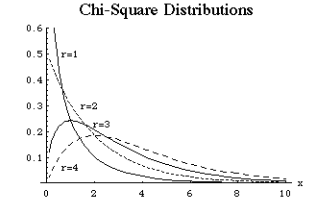
\includegraphics[width=\textwidth]{./chaps/23sec/images/1chi_square.png}
	\end{center}
	\caption{If $r\rightarrow\infty$ then chi-square distribution
	tends to normal distribution}
	\label{fig:23sec_chiSquared}
\end{figure}

\paragraph{Properties}
\subparagraph{Population}
If $X\hookrightarrow N(\mu, \sigma^{2}) \text{, then }\left( \frac{X-\mu}{\sigma} \right)^{2}\hookrightarrow\chi^{2}(1)$
\subparagraph{Sample} If $X\hookrightarrow N(\mu,\sigma^{2})\text{ and }\prth{X}{i}{1}{n}$ is a random sample from $X$, then:\\
$$ \su{{i=1}}{n}\left( \dfrac{X_{i}-\mu}{\sigma} \right)^{2}\hookrightarrow\chi^{2}(n)$$
\subparagraph{Sample variance} If $X\hookrightarrow N(\mu,\sigma^{2})\text{ and }\prth{X}{i}{1}{n}$ is a random sample from $X$, then:\\
$$ \dfrac{(n-1)S^{2}}{\sigma^{2}}\hookrightarrow\chi^{2}(n-1)$$
\subparagraph{Gamma} IF $X\hookrightarrow \gamma(\theta,\alpha)$, then:
$$ \dfrac{2}{\theta}\hookrightarrow\chi^{2}(2\alpha)$$

\section{Student's t-distribution}
\paragraph{Definition}
A continuous random variable $X$ is said to have a $t$-distribution 
with $\nu$ degrees of freedom if its probability density function is of
the form:
$$
f(x;\nu) = 
\dfrac{\Gamma\left(\frac{\nu+1}{2}\right)}{\sqrt{\pi\nu}~\Gamma\left(\frac{\nu}{2}\right)\left(1+\frac{x^{2}}{\nu}\right)^{\left(\frac{\nu+1}{2}\right)}}, -\infty\leq x\leq\infty
$$
where $\nu > 0$. If $X$ has a $t$-distribution with $\nu$ degrees of 
freedom, then we denote it by writing $X\hookrightarrow t(\nu)$\\
The distribution is a generalization of the Cauchy distribution and the
normal distribution:
$$
\left\{
\begin{array}{ll}
\nu=1 \Rightarrow \forall x\in \mathbb{R} & f(x;\nu) = \dfrac{1}{\pi(1+x^{2})}\\
\nu\rightarrow\infty \Rightarrow \forall x\in \mathbb{R} & \lm{\nu}{\infty} f(x;\nu) = \dfrac{1}{2\pi}e^{-\frac{1}{2}x^{2}}
\end{array}
\right.
$$
\paragraph{Properties}
\subparagraph{Expected value and Variance}
If the random variable $X$ has a $t$-distribution with $\nu$ degrees of
freedom, then:
$$
\mathbb{E}(X) = 
	\left\{
	\begin{array}{ll}
	0 & \mbox{if } \nu \geq 2\\
	DNE & \mbox{if } \nu = 1
	\end{array}
	\right.
$$
$$
\mathbb{V}(X) = 
	\left\{
	\begin{array}{ll}
		\dfrac{\nu}{\nu-2} & \mbox{if } \nu \geq 3\\
		DNE & \mbox{if } \nu \in \inter{1}{2} 
	\end{array}
	\right.
$$
\subparagraph{Normal and Chi-Squared distribution}
$$
\begin{cases}
Z\hookrightarrow N(0,1)\\
U\hookrightarrow\chi^{2}(\nu)\\
Z\text{ and }U\text{ independents}
\end{cases}
\Rightarrow
W=\dfrac{Z}{\sqrt{\frac{U}{\nu}}}\hookrightarrow t(\nu)
$$
\subparagraph{Normal variable sample}
$$
\begin{cases}
X\hookrightarrow N(\mu,\sigma^{2})\\
\prth{X}{i}{1}{n}\text{ a sample of the population }X
\end{cases}
\Rightarrow
\dfrac{\overline{X}-\mu}{\frac{S}{\sqrt{n}}}\hookrightarrow t(n-1)
$$

\section{Snedecor's F-distribution}
\paragraph{Definition}
A continuous random variable is said to have a $F$-distribution with
$\nu_{1}$ et $\nu_{2}$ degrees of freedom if its probability density
function is of the form:
$$
f(x,\nu_{1},\nu_{2})=
\left\{
\begin{array}{ll}
	\dfrac{\Gamma\left(\frac{\nu_{1}+\nu_{2}}{2}\right)\left(\frac{\nu_{1}}{\nu_{2}}\right)^{\frac{\nu_{1}}{2}}x^{\frac{\nu_{1}}{2}-1}}{\Gamma\left(\frac{\nu_{1}}{2}\right)\Gamma\left(\frac{\nu_{2}}{2}\right)\left(1+\frac{\nu_{1}}{\nu_{2}}x\right)^{\left(\frac{\nu_{1}+\nu_{2}}{2}\right)}} & \mbox{if } 0\leq x < \infty\\
	0 & \mbox{otherwise}
\end{array}
\right.
$$
The $F$-distribution was named in honor of Sir Ronald Fisher by George
Snedecor. $F$-distribution arises as the distribution of a ratio of 
variances.
\begin{figure}[H]
	\begin{center}
		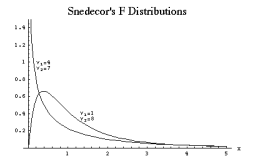
\includegraphics[width=.5\textwidth]{./chaps/23sec/images/2Snedecor_F_distribution.png}
	\end{center}
	\caption{Shape of the graph of $F$-distribution for various degrees of freedom.}
	\label{fig:23sec_F_distribution}
\end{figure}
\paragraph{Properties}
\subparagraph{Expected value and Variance}
$X\hookrightarrow F(\nu_{{1},nu_{2}})\Rightarrow$
$$
E(X) = 
\left\{
\begin{array}{ll}
	\frac{nu_{2}}{nu_{2}-2} & \mbox{if }\nu_{2}\geq 3 \\
	DNE &\mbox{if }\nu_{2}\in\inter{1}{2}
\end{array}
\right.
$$
\begin{center}
	And
\end{center}
$$
V(X) = 
\left\{
\begin{array}{ll}
	\frac{2\nu_{2}^{2}(\nu_{1}+\nu_{2}-2)}{\nu_{1}(\nu_{2}-2)^{2}(\nu_{2}-4)} & \mbox{if }\nu_{2}\geq 5 \\
	DNE &\mbox{if }\nu_{2}\in\inter{1}{4}
\end{array}
\right.
$$
\subparagraph{Inverse}
$X\hookrightarrow F(\nu_{1},\nu_{2})\Rightarrow \frac{1}{X}\hookrightarrow F(\nu_{2},\nu_{1})$\\
\subparagraph{Chi-squared and $F$-distributions}
$
\begin{cases}
	U\hookrightarrow\chi_{2}(\nu_{1})\\
	V\hookrightarrow\chi_{2}(\nu_{2})\\
	U\& V independent
\end{cases}
\Rightarrow
\dfrac{\frac{U}{\nu_{1}}}{\frac{V}{\nu_{2}}}\hookrightarrow F(\nu_{1},\nu_{2})
$
\subparagraph{Quotient of Inverses}
Let $X\hookrightarrow N(\mu_{1},\sigma_{1}^{2})\text{ and }\prth{X}{i}{1}{n}$ be a random sample of size $n$ from the population $X$.
Let $Y\hookrightarrow N(\mu_{2},\sigma_{2}^{2})\text{ and }\prth{Y}{i}{1}{m}$ be a random sample of size $n$ from the population $Y$.
$$
\dfrac{\frac{S_{1}^{2}}{\sigma_{1}^{2}}}{\frac{S_{2}^{2}}{\sigma_{2}^{2}}} \hookrightarrow F(n-1, m-1)
$$
where $S_{1}^{2}$, and $S_{2}^{2}$ denote the sample variances of the
first and second sample, respectively.


\chapter{Some Techniques for finding point Estimators of Parameters}
In point estimation, we try to find the parameter $\theta$ of the
population distribution $f(x;\theta)$ from the sample information. 
Thus, in the parametric point estimation one assumes the functional 
form of the pdf $f(x;\theta)$ to be known and only estimate the unknown
parameter $\theta$ of the population using information available from
the sample.
\section{Moment Method}
\paragraph{Parameter space}
Let $X$ be a population with the density function $f(x;\theta)$, where
$\theta$ is an unknown parameter. The set of all admissible values of 
$\theta$ is called a parameter space and it is denoted by $\Omega$ that
is:
$$
\Omega = \left\{\theta\in\mathbb{R}^{n}|f(x;\theta)\text{ is a pdf}\right\}
$$

\paragraph{Estimators}
Let $X\hookrightarrow f(x;\theta)$ and $\prth{X}{i}{1}{n}$ be a random
sample from population $X$. Any statistic that can be used to guess
the parameter $\theta$ is called an estimator of $\theta$. The 
numerical value of this statistic is called an estimate of $\theta$.\\
The estimator of the parameter $\theta$ is denoted by $\hat{\theta}$

\paragraph{Moment method}
Let $\prth{X}{i}{1}{n}$ be a random sample from a population $X$ with
probability density function $f\left(x;\prth{\theta}{j}{1}{m}\right)$
where $\prth{\theta}{j}{1}{m}$ are $m$ unknown parameters.\\
Let:
$\E{X^{k}}=\Su{-\infty}{\infty}x^{k}f\left(x;\prth{\theta}{j}{1}{m}\right)dx$ is the $k^{\text{th}}$ population moment about 0. Further, let
$M_{k}=\dfrac{1}{n}\su{{i=1}}{n}X_{i}^{k}$ be the $k^{\text{th}}$ 
sample moment about 0.\\
Then we find the estimator for the parameters $\prth{\theta}{j}{1}{m}$
by equating the first $m$ population moments (if they exist) to the
first $m$ sample moments that is:
$$
\left\{
\begin{array}{cc}
	\E{X}&= M_{1}\\
	\E{X^{2}}&= M_{2}\\
	\E{X^{3}}&= M_{3}\\
	&.\\
	&.\\
	&.\\
	\E{X^{m}}&= M_{m}

\end{array}
\right.
$$
The motivation of moment method comes from the fact that the sample 
moments are in some sense estimates for the population moments.

\section{Maximum Likelihood Method}
\paragraph{Definition}
Let $\prth{X}{i}{1}{n}$ be a random sample from a population $X$ with
probability density function $f(x;\theta)$, where $\theta$ is an
unknown parameter. The likelihood, $L(\theta)$, is the distribution of
the sample. That is:
$$
L(\theta) = \prd{{i=1}}{n}f(x_{i};\theta)
$$
The $\theta$ that maximizes the likelihood function $L(\theta)$ is
called the maximum likelihood estimator of $\theta$ and it is denoted
by $\hat{\theta}$

\paragraph{Method}
\begin{enumerate}
	\item Obtain a random sample $\prth{x}{i}{1}{n}$ from the
		distribution $X$ with probability density function
		$f(x;\theta)$
	\item Define the likelihood function for the sample 
		$\prth{x}{i}{1}{n}$ 
		by $L(\theta)=\prd{{i=1}}{n}f(x_{i};\theta)$
	\item find the expression for $\theta$ that maximizes 
		$L(\theta)$. This can be done directly or by maximizing
		$ln\left(L(\theta)\right))$
	\item replace $\theta$ by $\hat{\theta}$ to obtain an 
		expression for the maximum likelihood estimator for
		$\theta$
	\item find the observed value of this estimator for a given
		sample.
\end{enumerate}

\paragraph{Theorem}
Let $\hat{\theta}$ be a maximum likelihood estimator of a parameter
$\theta$ and let $g(\theta)$ be a function of $\theta$. Then the 
maximum likelihood estimator of $g(\theta)$ is given by 
$g\left(\hat{\theta}\right)$

\paragraph{Fisher information}
Let $X$ be an observation from a population with probability density 
function $f(x;\theta)$. Suppose $f(x;\theta)$ is continuous, twice
differentiable and it's support does not depend on $\theta$. Then the
Fisher information $I(\theta)$ in a single observation $X$ about 
$\theta$ is given by:
$$
I(\theta) = \Su{-\infty}{\infty}\left[\frac{d~ln\left(f(x;\theta)\right)}{d\theta}\right]^{2}f(x;\theta)dx
$$
It can be given alternatively as:
$$
I(\theta) = -\Su{-\infty}{\infty}\left[\frac{d^{2}~ln\left(f(x;\theta)\right)}{d\theta^{2}}\right]f(x;\theta)dx
$$
$
\begin{cases}
	\prth{X}{i}{1}{n}\text{ random sample from }X\\
	X\hookrightarrow f(x;\theta)
\end{cases}
\Rightarrow I_{n}(\theta) = nI(\theta)
$
\paragraph{Theorem}
Under certain regularity conditions on the $f(x;\theta)$ the maximum
likelihood estimator $\hat{estimator}$ of $\theta$ based on a random
sample of size $n$ from a population $X$ with probability density 
$f(x;\theta)$ is asymptotically normally distributed with mean 
$\theta$ and variance $\frac{1}{nI(\theta)}$. That is :
$$
\hat{\theta}_{ML} \hookrightarrow N\left( \theta,\frac{1}{nI(\theta)} \right)\text{ as }n\rightarrow\infty
$$

\section{Bayesian Method}
\paragraph{Prior distribution}
Let $\prth{X}{i}{1}{n}$ be a random sample from a distribution with 
density $f(x/\theta)$, where $\theta$ is the unknown parameter to be
estimated. \tB{The probability density function of the random variable 
$\theta$ is called the prior distribution of $\theta$} and usually 
denoted by $h(\theta)$

\paragraph{Posterior distribution}
Let $\prth{X}{i}{1}{n}$ be a random sample from a distribution with
density $f(x/\theta)$, where $\theta$ is the unknown parameter to be
estimated. \tB{The conditional density, $k\left(\theta;\prth{x}{i}{1}{
n}\right)$, of $\theta$ given the sample $\prth{x}{i}{1}{n}$ is called
the posterior distribution of $\theta$.}

\paragraph{Squared and Absolute Error Loss}
Let $\prth{X}{i}{1}{n}$ be a random sample from a distribution with 
density $f(x/\theta)$, where $\theta$ is the unknown parameter to be
estimated. Let $\hat{\theta}$ of $\theta$:
$
\begin{cases}
	\mathcal{L}_{2}\left(\theta\right) = \left(\hat{\theta}-\theta\right)^{2}\text{ Squared error loss}\\
	\mathcal{L}_{1}\left(\theta\right) = \left|\hat{\theta}-\theta\right|\text{ Absolute error loss}
\end{cases}
$

\paragraph{Risk}
Let $\prth{X}{i}{1}{n}$ be a random sample from a distribution with 
density $f(x/\theta)$, where $\theta$ is the unknown parameter to be
estimated. Let $\hat{\theta}$ be an estimator of $\theta$ and let 
$\mathcal{L}\left(\hat{\theta}\right)$ be a given loss function. The 
expected value of this loss function with respect to the population 
distribution $f(x/\theta)$, that is
$R_{\mathcal{L}}(\theta)=\Su{}{}\mathcal{L}\left(\hat{\theta}\right)f(x/\theta)dx$\\
In Bayesian estimation of parameter one chooses an estimate 
$\hat{theta}$ for $\theta$ such that:
$k\left(\hat{\theta}/\prth{x}{i}{1}{n}\right)$ is maximum subject to a
loss function.\\
Mathematically this equivalent to minimizing the integral:
$\Su{\Omega}{}\mathcal{L}\left(\hat{\theta},\theta\right)k\left(\theta/\prth{x}{i}{1}{n}\right)d\theta$
where $\Omega$ denotes the support of the prior density $h(\theta)$ of
$\theta$.

\paragraph{Estimator for squared error}
Let $\prth{X}{i}{1}{n}$ be a random sample from a distribution with 
density $f(x/\theta)$, where $\theta$ is the unknown parameter to be
estimated. If the loss function is squared error, then the Bayes'
estimator $\hat{\theta}$ of parameter $\theta$ is given by:
$$\hat{\theta}=\E{\theta/\prth{x}{i}{1}{n}}$$
where the expectation is taken with respect to density $k\left(\theta/\prth{x}{i}{1}{n}\right)$

\paragraph{Estimator for absolute error}
Let $\prth{X}{i}{1}{n}$ be a random sample from a distribution with 
density $f(x/\theta)$, where $\theta$ is the unknown parameter to be
estimated. If the loss function is absolute error, then the Bayes'
estimator $\hat{\theta}$ of parameter $\theta$ is given by:
$$\hat{\theta}=\text{ median of }k\left(\theta/\prth{x}{i}{1}{n}\right)$$
where $k\left(\theta/\prth{x}{i}{1}{n}\right)$ is the posterior distribution.

\section{Information Theory}
Aim: representing data in a compact fashion.\\
Note that compactly representing data requires allocating short codewords to 
highly probable bit strings, and reserving longer codewords to less probable
bit strings.

\paragraph{Entropy}
The \textbf{entropy} is a measure of its uncertainty, $\mathbb{H}(X)$
\begin{center}
	$\mathbb{H}(X) \triangleq - \su{{k=1}}{K}\Prob{X=k}\log_{2}(
	\Prob{X=k})$
\end{center}

\paragraph{KL Divergence}
\paragraph{Equality}
Kullback-Leibler divergence or \textbf{relative entropy} allows to measure
the dissimilarity of 2 probability distribution $p$ and $q$.\\
\begin{align*}
	\mathbb{KL}(p||q) &\triangleq \su{{k=1}}{k}p_{k}\log\left(
\dfrac{p_{k}}{q_{k}}\right)\\
	&= \su{k}{}p_{k}\log\left(p_{k}\right) - \su{k}{}p_{k}\log\left(q_{k}
	\right)\\
	&=  -\mathbb{H}(p) + \underbrace{\mathbb{H}(p,q)}_{\text{cross 
	entropy}}
\end{align*}


\paragraph{Inequality}
Let $(p,q)$ 2 distinct probability distributions 
$\begin{cases}
	\mathbb{KL} \geq 0 \\
	p=q \Rightarrow \mathbb{KL} = 0
\end{cases}$
\paragraph{Mutual Information}
\subparagraph{Definition}
Aim: knowing how much knowing one varaible tells us about one other.
Motivation: The correlation coefficient is only defined for real-valued variables and has some limitations. 
Purpose: Determining how similar the joint distribution $p(X, Y)$ is to the factored 
distribution $p(X), p(Y)$
\begin{align*}
    \mathcal{I}(X:Y) &\triangleq \mathcal{KL}(p(X, Y) || p(X), p(Y)) \\
                     &= \su{x}{}\su{y}{}p(x, y)\log\left(\dfrac{p(x,y)}{p(x)p(y)}\right)
\end{align*}
\subparagraph{Pointwise Mutual Information}
This measures the discripencey between these events occuring together compared to what 
would be expected by chance. MI is indeed the expected value of the PMI\\
$PMI(x, y) = \log\left(\dfrac{p(x, y)}{p(x)p(y)}\right) = \log\left(\dfrac{p(x|y)}
{p(x)}\right) = \log\left(\dfrac{p(y|x)} {p(y)}\right)$a\\
This is the amount we learn from updating the prior $p(x)$ into the posterior $p(x|y)$, 
or equivalently updating the prior $p(y)$ into the posterior $p(y|x)$.

\subparagraph{Maximal Information Coefficient}
For continuous random variables, it is common to \textbf{discretize} by dividing the 
ranges of each variable into bins. As the bin boundaries can have a significant impact, we
can try many different bin sizes and location, then compute the maximum MI achieved.
This statistic, appropriately normalized, is known as the Maximal Information Coefficient
(MIC).\\

$MIC \triangleq \displaystyle\max_{x,y:xy<B} \dfrac{\max_{G\in\mathcal{G}(x,y)}\mathcal{I}(X(G):Y(G))}{\log(\min(x,y))}$


\chapter{Criteria for evaluating the Goodness of Estimators}
\section{The Unbiased Estimator}
\paragraph{The Unbiased Estimator}
$\hat{\theta} =\text{ unbiased estimator of }\theta \Leftrightarrow
\E{\hat{\theta}}=\theta$\\
In statistics between 2 unbiased estimators one prefers the estimator
which has the minimum variance. \\
There are 2 disadvantages:
\begin{enumerate}
	\item A unbiased estimator for a parameter may not exist.
	\item Unbiasedness is not invariant under functional 
		transformation.
\end{enumerate}

\section{The relatively Efficient Estimator}
\paragraph{Efficiency of estimators}
Let $\hat{\theta}_{1}$ and $\hat{\theta}_{2}$ be 2 unbiased estimators
of $\theta$.\\
$$\V{\hat{\theta}_{1}} < \V{\hat{\theta}_{2}} \Rightarrow 
\hat{\theta}_{1}\text{ is said to be more efficient than }\hat{\theta}_{2}$$ \\
The ratio is given by:
$$ \eta\left(\hat{\theta}_{1},\hat{\theta}_{2}\right)=\dfrac{\V{\hat{\theta}_{2}}}{\V{\hat{\theta}_{1}}}$$
is called relative efficiently of $\hat{\theta}_{1}$ with respect to 
$\hat{\theta}_{2}$.

\section{The Minimun Variance Unbiased Estimator}
\paragraph{Definition}
Let $\hat{\theta}$ to be an unbiased estimator of $\theta$
For any unbiased estimator $\hat{T}$ of $\theta$:
$\V{\hat{\theta}} \leq \V{\hat{T}} \Leftrightarrow 
\hat{\theta}$ is said to be a uniform minimum variance unbiased
estimator of $\theta$.

\paragraph{Definition (2)}
Let $\hat{\theta}$ to be an unbiased estimator of $\theta$.
$\hat{\theta}$ minimizes the variance $\E{\left[\hat{\theta}-\theta\right]^{2}} \Rightarrow \hat{\theta}$ is said to be a minimum variance 
unbiased estimator.

\paragraph{Minoration of an unbiased estimator}
$
\text{For any }h\left(\prth{x}{i}{1}{n}\right)\text{ with }
\E{h\left(\prth{x}{i}{1}{n}\right)}<\infty
$
$$
\begin{cases}
	X\text{ a population with pdf }f(x;\theta)\\
	\prth{X}{i}{1}{n}\text{ a random sample of size }n\text{ from
	X}\\
	\hat{\theta}\text{ any unbiased estimator of }\theta\\
	L(\theta)\text{ the likelihood function is differentiable}\\
	\dfrac{d}{d\theta}\Su{-\infty}{\infty}\cdots\Su{-\infty}{\infty}h\left(\prth{x}{i}{1}{n}\right)L(\theta)dx_{1}\cdots dx_{n} = 
	\Su{-\infty}{\infty}\cdots\Su{-\infty}{\infty}h\left(\prth{x}{i}{1}{n}\right)\dfrac{d}{d\theta}L(\theta)dx_{1}\cdots dx_{n}
\end{cases}
$$

$$
\Rightarrow
\V{\hat{\theta}} \geq \dfrac{1}{\E{\left[\frac{\partial~ln\left(L(\theta)\right)}{\partial\theta}\right]^{2}}}
$$
If $L(\theta)$ is twice differentiable with respect to $\theta$, the
last inequality can be stated equivalently as 
$
\V{\hat{\theta}} \geq \dfrac{-1}{\E{\frac{\partial^{2}~ln\left(L(\theta)\right)}{\partial\theta^{2}}}}
$
\paragraph{Theorem}
$
\begin{cases}
	X\text{ a population with pdf }f(x;\theta)\\
	\prth{X}{i}{1}{n}\text{ a random sample of size }n\text{ from
	X}\\
	\hat{\theta}\text{ an unbiased estimator}\\
	\V{\hat{\theta}} = \dfrac{1}{\E{\left[\frac{\partial~ln\left(L(\theta)\right)}{\partial\theta}\right]^{2}}}

\end{cases}\\
\Rightarrow 
\hat{\theta}
$ is a minimum variance unbiased estimator of $\theta$

\paragraph{Cramér-Rao lower bound} 
Let $\hat{\theta}$ to be a unbiased estimator.\\ 
$
\V{\hat{\theta}} = \dfrac{1}{\E{\left[\frac{\partial~ln\left(L(\theta)\right)}{\partial\theta}\right]^{2}}}
\Rightarrow
\hat{\theta}
$
is an efficient estimator

\section{Sufficient Estimator}
\paragraph{Definition}
$
\begin{cases}
	X\hookrightarrow f(x;\theta) be a population\\
	\prth{X}{i}{1}{n}\text{ random sample of }X\\
	\hat{\theta}\text{ an estimator of }\theta\\
	\text{ the conditional distribution of the sample given }\hat{\theta}\text{ does not depend on the parameter }\theta
\end{cases}\\
\Rightarrow
\hat{\theta}
$
is a \emph{sufficient estimator}

\paragraph{Theorem}
$
\begin{cases}
	X\hookrightarrow f(x;\theta) be a population\\
	\prth{X}{i}{1}{n}\hookrightarrow f\left(\prth{x}{i}{1}{n};\theta\right)\\
	f\left(\prth{x}{i}{1}{n};\theta\right)=\phi\left(\hat{\theta},\theta\right)h\left(\prth{x}{i}{1}{n}\right)\\
\end{cases}\\
\Rightarrow
\hat{\theta}
$
is sufficient for $\theta$

\paragraph{Theorem}
$
\begin{cases}
	X\hookrightarrow f(x;\theta)=e^{\left\{K(x)A(\theta)+S(x)+B(\theta)\right\}}\\
	\prth{X}{i}{1}{n}\text{ a random sample from }X
\end{cases}\\
\Rightarrow
\text{the statistic }\su{{i=1}}{n}K(X_{i})
$ is a sufficient statistic for the parameter $\theta$

\paragraph{Necessary estimator}
$\hat{\theta}$ can be written as a function of every sufficient
estimators $\Rightarrow$ $\hat{\theta}$ is a \emph{necessary estimator}

\section{Consistent Estimator}
\paragraph{Consistent sequence of estimators}
$
\begin{cases}
	X\hookrightarrow f(x;\theta)\text{ a population}\\
	\prth{X}{i}{1}{n}\text{ a sample from }X\\
	\left\{\theta_{n}\right\}\text{ a sequence of estimators}\\
	\forall\epsilon>0,\lm{n}{\infty}\Prob{\left|\hat{\theta}_{n}-\theta\right|\geq \epsilon}=0
\end{cases}\\
\Rightarrow
\left\{\theta_{n}\right\}
$ is said to be \emph{consistent} for $\theta$

\paragraph{Theorem}
$
\begin{cases}
	X\hookrightarrow f(x;\theta)\text{ a population}\\
	\prth{X}{i}{1}{n}\text{ a sample from }X\\
	\left\{\theta_{n}\right\}\text{ a sequence of estimators}\\
	\forall n\in\mathbb{N},\V{\hat{\theta}_{n}}<\infty\\
	\lm{n}{\infty}\E{\left[\hat{\theta}_{n}-\theta\right]^{2}}=0
\end{cases}
\Rightarrow
\forall\epsilon >0 \lm{n}{\infty}\Prob{\left|\hat{\theta}_{n}-\theta\right|\geq \epsilon} = 0
$

\paragraph{Limit of a sequence variance}
$
\begin{cases}
	X\hookrightarrow f(x;\theta)\\
	\prth{X}{i}{1}{n}\text{ be a random sample from }X\\
	\left\{\hat{\theta}_{n}\right\}\text{ a sequence of estimators of }\theta\text{ based on the sample}\\
	\forall n\in\mathbb{N},\V{\hat{\theta}_{n}}\leq \infty
\end{cases}\\
\Rightarrow
\lm{n}{\infty}\E{\left[\hat{\theta}_{n}-\theta\right]^{2}}=0
$


\part{Tests}
\chapter{Some Techniques for finding Interval Estimators of Parameters}
\section{Interval Estimators and Confidence Intervals for Parameters}
\paragraph{Interval estimator \& Interval estimate}
Let $\prth{X}{i}{1}{n}$ be a random sample from $X\hookrightarrow f(x;\theta)$.\\
The \emph{interval estimator} of $\theta$ is a pair of statistics $L=
L(\prth{X}{i}{1}{n})\text{ and }U=U(\prth{X}{i}{1}{n})\text{ with }
L\leq U$ such that if $\prth{x}{i}{1}{n}$ is a set of sample data, then
$\theta$ belongs to the interval $\left[L(\prth{X}{i}{1}{n}),U(\prth{X}{i}{1}{n})\right]$\\
The interval $[l,u]$ will be denoted as an interval estimate of $\theta$ of $\theta$ whereas the random interval [L,U] will denote the 
interval estimator of $\theta$

\paragraph{Confidence interval}
$
\begin{cases}
	X\hookrightarrow f(x;\theta)\\
	\prth{X}{i}{1}{n}\text{ a random sample from }X\\
	\Prob{L\leq\theta\leq U}=1-\alpha
\end{cases}\\
\Rightarrow
$ The interval estimator of $\theta$ is called a $100(1-\alpha)\%$ 
\emph{confidence interval} for $\theta$

\section{Pivotal Quantity Method}
\paragraph{Definition}
Let $\prth{X}{i}{1}{n}$ be a random sample from $X\hookrightarrow f(x;
\theta)$.\\
A \emph{pivotal quantity} $Q$ is a function of $\prth{X}{i}{1}{n}$ and
$\theta$ \emph{whose pdf is independent of the parameter} $\theta$

\paragraph{Location-scale family}
$
g:\mathbb{R}\rightarrow\mathbb{R}\text{ a pdf}\\
\Rightarrow
\mathcal{F}=\left\{f(x;\mu;\sigma)=\frac{1}{\sigma}g\left(\frac{x-\mu}{\sigma}\right)|(\mu,\sigma)\in\mathbb{R}\times\mathbb{R}_{+}^{*}\right\}
$ is called the \emph{location-scale family} with standard probability
function density $f(x;\theta)$\\
The parameter $\mu$ is called the \emph{location parameter} and the 
parameter $\sigma$ is called the \emph{scale parameter}.\\
$\sigma = 1 \Rightarrow \mathcal{F}$ is called \emph{location} family\\
$\mu = 0 \Rightarrow \mathcal{F}$ is called \emph{scale} family

\paragraph{Remark}
Let be $\hat{\mu}\text{ and }\hat{\sigma}$ respectively the maximum
likelihood of $\mu\text{ and }\sigma$:\\
Density $\in$ \emph{location} family $\Rightarrow \hat{\mu}-\mu\text{ is the pivot for }\mu$\\
Density $\in$ \emph{scale} family $\Rightarrow
	\frac{\hat{\sigma}}{\sigma}\text{ is the pivot for }\sigma $\\ 
Density $\in$ \emph{location-scale} family $\Rightarrow
\begin{cases}
	\frac{\hat{\mu}-\mu}{\hat{\sigma}}\text{ is the pivot for }\mu\\
	\frac{\hat{\sigma}}{\sigma}\text{ is the pivot for }\sigma
\end{cases}
$ 


\section{Confidence Interval for Population Mean}
Practice exercises

\section{Confidence Interval for Population Variance}
Practice exercises

\section{Confidence Interval for Parameter of some Distribution not belonging to the Location-Scale Family}
\begin{itemize}
	\item
\end{itemize}

\section{Approximate Confidence Interval for Parameter with MLE}
\begin{itemize}
	\item
\end{itemize}

\section{The Statistical or General Method}
\begin{itemize}
	\item
\end{itemize}

\section{Criteria for Evaluating Confidence Intervals}
\begin{itemize}
	\item
\end{itemize}


\chapter{Test of Statistical Hypotheses}
\section{Introduction}
\paragraph{Statistical hypothesis}
is a conjecture about the distribution $f(x;\theta)$ of a population
$X$.\\
This conjecture is usually about the parameter $\theta$.

\paragraph{Simple and Composite hypotheses}
H completely specifies the density $f(x;\theta)$ of the population 
$\Rightarrow$ H is \emph{simple hypothesis}\\
H does not completely specify the density $f(x;\theta)$ of the
population $\Rightarrow$ H is \emph{composite hypothesis}

\paragraph{Null and alternative hypothesis}
Null hypothesis $H_{0}$ is to be tested, and correspond to the idea
that an observed difference is due to chance.\\
Alternative hypothesis $H_{a} = \overline{H_{0}}$, corresponds to the
idea that the observed difference is real.

\paragraph{Hypothesis test}
It is used to measure the difference between the data and what is
expected on the null hypothesis.\\
Let $X\hookrightarrow f(x;\theta)\text{ and }\prth{X}{i}{1}{n}$ a 
sample from $X$ and $C$ a Borel set in $\mathbb{R}^{n}$
It is an ordered sequence: $\left(\prth{X}{i}{1}{n};H_{0},H_{\alpha},C\right)$\\
The set $C$ is called the \emph{critical region} in the hypothesis 
test. The critical region is obtained using a \emph{test statistics}
$W\left(\prth{X}{i}{1}{n}\right)$. If the outcome of 
$\prth{X}{i}{1}{n}$ turns out to be an element of $C$ then we decide to
accept $H_{\alpha}$ otherwise we accept $H_{0}$

\section{Tests}
\paragraph{Z-test}
It says how many SEs away an observed value is from its expected value,
where the expected value is calculated using the null hypothesis.
\begin{center}
	$z=\dfrac{\text{observed}-\text{expected}}{\text{SE}}$
\end{center}
\paragraph{T-test}
\begin{center}
	$t=\dfrac{\text{average of draws}-\text{c}}{\text{SE}}$
\end{center}
$c$ corresponding to the constant which is fixed in $H_{0}$\\
As the number degrees of freedom increases the curves get closer and 
closer to the normal.
\paragraph{Test Method}
\begin{figure}[H]
	\begin{center}
		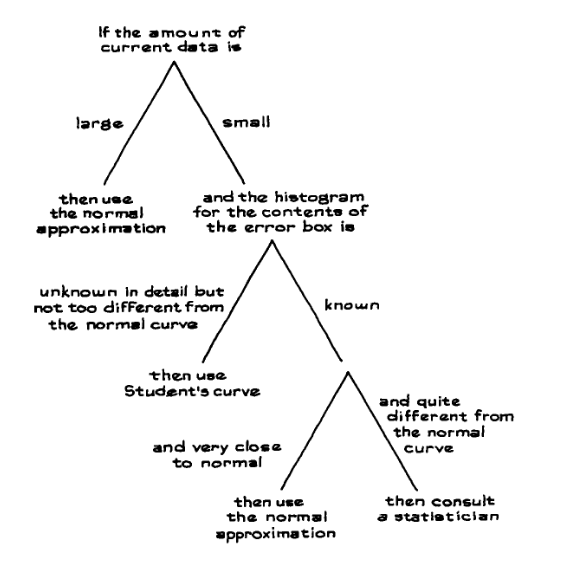
\includegraphics[width=.5\textwidth]{./chaps/27sec/images/1_methodApproxNorm.png}
	\end{center}
	\caption{Procedure when testing}
	\label{fig:1_mehtodeApproxNorm}
\end{figure}

\section{A method of Finding Tests}
\paragraph{The likelihood ratio test statistics}
For testing the simple null hypothesis $H_{0}:\theta\in\Sigma_{0}$ 
against the composite alternative hypothesis $H_{\alpha}\notin\Sigma_{0}$ based on a set of random sample data $\prth{x}{i}{1}{n}$ is defined
as $W\left(\prth{x}{i}{1}{n}\right) = \frac{\max_{{\theta\in\Omega_{0}}}L\left(\theta;\prth{x}{i}{1}{n}\right)}{\max_{\theta\in\Omega}L\left(\theta;\prth{x}{i}{1}{n}\right)}$ \\
Let $k\in[0,1]$ a likelihood ratio test is any test that has a critical
region $C$ that is rejection region) of the form:
$C=\left\{\prth{x}{i}{1}{n}|W\left(\prth{x}{i}{1}{n}\right)\leq k\right\}$

\section{Methods of Evaluating Tests}
\begin{tabular}{|c|c|c|}
	\hline
	& $H_{0}$ is true & $H_{0}$ is false\\
	\hline
	Accept $H_{0}$ & Correct Decision & Type $II$ Error\\
	\hline
	Reject $H_{0}$ & Type $I$ Error & Correct Decision\\
	\hline
\end{tabular}

\paragraph{Significance level}
It is denoted by $\alpha = \Prob{\text{Type I Error}}$ corresponds to
the probability of getting a test statistic as extreme as, or more 
extreme than the observed one. This probability is computed on the 
basis that the $H_{0}$ is true.

\paragraph{P-value}
Is the probability of getting a big test statistic, assuming the null
hypothesis to be right.
\paragraph{Probability of type II error}
It is denoted by $\beta = \ProbC{H_{0}\text{ is false}}{\text{Accept }H_{0}} = \ProbC{H_{\alpha}\text{ is true}}{\text{Accept }H_{0}}$ 

\paragraph{The power function}
It is the function $\pi : \Omega\rightarrow [0,1]$ defined by:
$
\pi(\theta)=
\begin{cases}
	\Prob{\text{Type I Error}}\\
	1-\Prob{\text{Type II Error}}
\end{cases}
$

\paragraph{A test of level $\delta$} Given $\delta\in[0,1]$
$\max_{\theta\in\Omega_{0}}\pi(\theta)\leq\delta$
\paragraph{Test of size $\delta$} Given $\delta\in[0,1]$
$\max_{\theta\in\Omega_{0}}\pi(\theta)=\delta$
\paragraph{Uniformly most powerful} 
Let $T$ be a test procedure for testing the null hypothesis.
For any test $W$ of level $\delta,\\ \forall\theta\in\Omega_{0}, \pi_{T}(\theta)\geq\pi_{W}(\theta)$ 

\paragraph{Theorem Neyman-Perarson}
$
\begin{cases}
	X\hookrightarrow f(x;\theta)\\
	\prth{X}{i}{1}{n}\text{ sample from }X\\
	L\left(\theta;\prth{x}{i}{1}{n}=\prd{{i=1}}{n}f(x_{i};\theta)\right)\text{ likelihood function of the sample }
\end{cases}\\
\Rightarrow
C=\left\{\prth{x}{i}{1}{n}|\frac{L\left(\theta_{0},\prth{x}{i}{1}{n}\right)}{L\left(\theta_{\alpha},\prth{x}{i}{1}{n}\right)}\right\}\leq k
$ for $k\in\mathbb{R}_{+}^{*}$ is best of its size for testing:\\
$H_{0}: \theta = \theta_{0}$ against $H_{a}:\theta = \theta_{a}$

\section{Some Examples of Likelihood Ratio Tests}
\begin{itemize}
	\item
\end{itemize}


\chapter{Simple Linear Regression and Correlation Analysis}
\section{Least Squared Method}
\paragraph{Unbiased estimators}
\begin{enumerate}
	\item $\E{Y_{x}}=a+\beta x$ so that $\mu_{i}=\E{Y_{i}}=\alpha+
		\beta x_{i}$
	\item $\prth{Y}{i}{1}{n}$ are independent;
	\item $\prth{Y}{i}{1}{n}$ has the same variance $\sigma^{2}$
\end{enumerate}
$\E{Y/X}=\alpha + \beta x$ are unbiased.

\section{Normal Regression Analysis}
\paragraph{Likelihood estimators}
In the normal regression analysis, the likelihood estimators 
$\hat{\beta}\text{ and }\hat{\alpha}$ are unbiased estimators of
$\beta\text{ and }\alpha$ respectively.

\paragraph{Distributions of the estimators}
In the normal regression analysis, the distributions of the estimators
$\hat{\beta}$ and $\hat{\alpha}$ are given by:\\
$
\begin{cases}
	\hat{\beta}\hookrightarrow \mathbb{N}\left(\beta,\dfrac{\sigma^{2}}{S_{xx}}\right)\\
	\hat{\alpha}\hookrightarrow \mathbb{N}\left(\alpha,\dfrac{\sigma^{2}}{n}+\dfrac{\overline{x}^{2}\sigma^{2}}{S_{xx}}\right)
\end{cases}
$

\section{The Correlation Analysis}
\paragraph{Correlation coefficient}
$\left(\left(X_{i},Y_{i}\right)_{1\leq i\leq n}\right)\text{ from }
\left(X,Y\right) \Rightarrow
\text{ Sample correlation coefficient is defined as }\\
R = \dfrac{\su{{i=1}}{n}\left(X_{i}-\overline{X}\right)\left(Y_{i}-\overline{Y}\right)}{\sqrt{\su{{i=1}}{n}\left(X_{i}-\overline{X}^{2}\right)}\sqrt{\su{{i=1}}{n}\left(Y_{i}-\overline{Y}^{2}\right)}}$\\
And $-1\leq R\leq 1$


\chapter{Analysis of Variance}
\section{One-way Analysis of Variance with Equal Sample Sizes}
\paragraph{Theorem ANOVA}
$
\begin{cases}
	\text{Model is given by } \forall (i,j)\in\inter{1}{m}\times\inter{1}{n}Y_{ij}=\mu_{i}+\epsilon_{ij}\\
	\left(\epsilon_{ij}\right)_{(i,j)\in\inter{1}{m}\times\inter{1}{n}}\text{ are independent and normally distributed}
\end{cases}\\
\Rightarrow
\begin{cases}
	\hat{\mu_{i}}=\overline{Y}_{i\bullet} = \dfrac{1}{n}\su{{j=1}}{n}Y_{ij}\\
	\hat{\sigma^{2}} = \frac{1}{nm}SS_{W} = \frac{1}{mn}\su{ {i=1}}{m}\su{{j=1}}{n}\left( Y_{ij}-\overline{Y}_{i\bullet} \right)^{2}
\end{cases}
$

\paragraph{Lemma}
$
\begin{cases}
	\overline{Y}_{\bullet\bullet}=\dfrac{1}{nm}\su{{i=1}}{m}\su{{j=1}}{n}Y_{ij}\\
	SS_{T}=\dfrac{1}{nm}\su{{i=1}}{m}\su{{j=1}}{n}\left(Y_{ij}-\overline{Y}_{\bullet\bullet}\right)^{2}\\
	SS_{W}=\dfrac{1}{nm}\su{{i=1}}{m}\su{{j=1}}{n}\left(Y_{ij}-\overline{Y}_{i\bullet}\right)\\
	SS_{B}=\dfrac{1}{nm}\su{{i=1}}{m}\su{{j=1}}{n}\left(Y_{i\bullet}-\overline{Y}_{\bullet\bullet}\right)^{2}\\
\end{cases}
\Rightarrow
SS_{T}=SS_{W}+SS_{B}
$
\paragraph{ANOVA model}
Consider ANOVA model:
$
\begin{cases}
\forall (i,j)\in\inter{1}{m}\times\inter{1}{n}Y_{ij}=\mu_{i}+\epsilon_{ij}\\
Y_{ij}\hookrightarrow\mathbb{N}(\mu_{i},\sigma^{2})
\end{cases}
\Rightarrow
\begin{cases}
	\text{(a) the random variable }\frac{SS_{W}}{\sigma^{2}}\hookrightarrow \chi^{2}\left(m(n-1)\right)\\
	\text{(a) the statics }SS_{W}\text{ and }SS_{B}\text{ are independent}\\
	H_{0}:\forall (i,j)\in\inter{1}{m}^{2} \mu_{i}=\mu_{j}\text{ it is True}
\end{cases}
\Rightarrow
\begin{cases}
	\text{the random variable }\frac{SS_{B}}{\sigma^{2}}\hookrightarrow\chi^{2}(m-1)\\
	\text{the statics }\frac{SS_{B}m(n-1)}{\sigma^{2}(m-1)}\hookrightarrow F(m-1,m(n-1))\\
	\text{the random variable }\frac{SS_{T}}{\sigma^{2}}\hookrightarrow \chi^{2}(nm-1)
\end{cases}
$


\section{One-way Analysis of Variance with Unequal Sample Sizes}
\begin{itemize}
	\item
\end{itemize}

\section{Pair Wise Comparisons}
\begin{itemize}
	\item
\end{itemize}

\section{Test for Homogeneity of Variances}
\begin{itemize}
	\item
\end{itemize}


\chapter{Goodness of Fits Tests}
\section{Chi-Squared test}
\begin{itemize}
	\item
\end{itemize}

\section{Kolmogorov-Smirnov test}
\begin{itemize}
	\item
\end{itemize}


\end{document}
